% 中文初稿。编译：xelatex main && bibtex main && xelatex main && xelatex main
% 图引用项目根目录的 figures/，表 1 由 experiments/make_table1.py 生成到 tables/table1.tex。
\documentclass[11pt,a4paper]{ctexart}
\usepackage[margin=2.4cm]{geometry}
\usepackage{amsmath,amssymb,bm}
\usepackage{graphicx}
\usepackage{booktabs}
\usepackage{xcolor}
\usepackage[numbers,sort&compress]{natbib}
\usepackage[colorlinks=true,linkcolor=blue!50!black,citecolor=blue!50!black,urlcolor=blue!50!black]{hyperref}
\graphicspath{{../figures/}}
% 放宽浮动体比例，避免图都被推到文末
\renewcommand{\topfraction}{0.9}
\renewcommand{\bottomfraction}{0.8}
\renewcommand{\textfraction}{0.1}
\renewcommand{\floatpagefraction}{0.8}
\setcounter{topnumber}{3}
\setcounter{totalnumber}{4}

\newcommand{\todo}[1]{\textcolor{red!70!black}{［待写：#1］}}
\newcommand{\Qint}{Q_\mathrm{int}}
\newcommand{\Qone}{Q_{\mathrm{ext},1}}
\newcommand{\Qtwo}{Q_{\mathrm{ext},2}}

\title{Kerr 微梳储备池能做到多好？\\谱相位输入掩模、噪声下限与软件对照}
\author{杜昌旭\\[2pt]
\small 上海理工大学\\
\small \href{mailto:yuzhuj520@gmail.com}{yuzhuj520@gmail.com}}
\date{初稿，\today}

\begin{document}
\maketitle

\begin{abstract}
Kerr 微梳储备池已有几种方案，但它们和软件比较的条件各不相同，所以在现实噪声下它最好能做到什么程度、被什么限制，还不清楚。
我们用 Lugiato--Lefever 模型的仿真回答这个问题。为了逼近上限，我们提出谱相位输入掩模：给与微环对齐的输入光梳的各根梳齿加上随机的复振幅偏置和调制权重，
让微环工作在输出由输入决定的相干种子区。在相同的器件参数、光功率、读出、噪声模型和选点预算下，它在 Mackey--Glass 预测上比单泵浦编码和整体调制的光梳好一到两个数量级，
起作用的是梳齿相位的随机性。逐项拆分噪声表明，理想探测器下的误差下限约一半来自失谐抖动、一半来自散粒噪声；
失谐抖动即使完全已知也无法在读出端扣除，因此激光本征线宽是硬指标，本文的器件要求在约 $5~\mathrm{kHz}$ 以下。
把软件储备池的输入噪声从零扫到 $3\times10^{-3}$，最好的单个微环相当于输入接约 7 位模数转换器的 31 节点回声状态网络，
低于微环工作速率下现成转换器的精度；把微环 31 路读数的量化也计入后，同样位数下软件仍然更好。所以在本文考察的任务上，微梳储备池的精度上限低于同规模软件，它的价值只能来自物理层。
\end{abstract}

\section{引言}\label{sec:intro}

储备池计算只训练一个线性读出层，把输入送进一个固定的非线性动力系统，让它把输入的历史展开成高维特征~\cite{jaeger2001,jaeger2004}。
因为动力系统本身不需要训练，它很适合用物理器件实现，光学是其中研究最多的方向之一~\cite{vandersande2017}。
频率复用的方案把一个光学腔的各根纵模当作储备池的节点，用一个腔、一组波长同时得到几十个特征~\cite{butschek2020,lupo2023}；
光学的下一代储备池计算也沿着类似的思路发展~\cite{cox2024,wang2025ngrc}。
Kerr 微环是这类方案的自然候选：它的四波混频把泵浦的能量转移到几十根梳齿上，提供了强的、片上的非线性，梳齿间隔又宽到可以逐根解复用读出。
近两年已有几种微梳储备池方案：调制泵浦功率、工作在混沌区的光梳~\cite{shishavan2025}，调制泵浦失谐、工作在单孤子态~\cite{cuevas2025}，
调制泵浦相位、工作在腔孤子态~\cite{arabieh2026soliton}，以及用同步脉冲串整体驱动的频率复用腔~\cite{arabieh2026pulse}。
它们有一个共同点：信号只通过一个自由度（泵浦的功率、失谐或相位，或者所有梳齿一起调制）进入器件。
这带来两个问题。在混沌区，梳齿由调制不稳定性从噪声中长出来，同样的输入两次给出的输出可能完全不同（第~\ref{sec:mechanism}~节）；
在孤子区，输出可以重复，但要把器件稳定在孤子存在的区间内，输入能施加的扰动也因此受限。

更根本的问题是，这些工作和软件比较的条件并不统一：工作点怎样选、在哪一次噪声实现上报告、给软件基线设多大的噪声，都各不相同，
而我们发现这几个选择中的任何一个都能让比较的结论翻转。
所以一个基本的问题还没有回答：\emph{在现实噪声下，Kerr 微梳储备池最好能做到什么程度？被什么限制？怎样和软件公平比较？}
只用一个输入自由度的方案离这个上限有多远，也就不清楚。

本文用仿真回答这个问题。为了逼近上限，我们提出谱相位输入掩模：把一个与微环对齐的输入光梳的 16 根梳齿各加上随机的复振幅偏置和调制权重，与泵浦一起送入微环。
输入梳齿本身就落在谐振上，边带由输入相干地“种”下去，所以微环工作在一个输出由输入决定的相干种子区。
我们在同一个仿真器、同样的器件参数和光功率范围、同样的读出、同样的噪声模型、同样的选点预算下，比较了八种编码，
并用多组独立的噪声实现选点和报告。主要结论如下：
\begin{enumerate}
\item \emph{编码决定能否接近上限}（第~\ref{sec:mechanism}、\ref{sec:encodings}~节）。谱相位掩模在 Mackey--Glass 预测上比单泵浦编码和整体调制的光梳好一到两个数量级，
      在信道均衡上小幅领先，在 NARMA-10 上单环不成立。起作用的是梳齿相位的随机性，实现上只需一个调制器加两个谱相位整形器。
\item \emph{上限由什么决定}（第~\ref{sec:noise}、\ref{sec:readout}~节）。理想探测器下的误差下限约一半来自失谐抖动、一半来自散粒噪声，换平台、加功率都降不了它。
      失谐抖动在读出端扣不掉，所以激光的本征线宽是硬指标：本文的器件要求在约 $5~\mathrm{kHz}$ 以下。读出侧的两种改法能把误差再降约 2 倍。
      微环贡献的是非线性特征而不是记忆，记忆要靠外加的延迟线。
\item \emph{上限在软件坐标里的位置}（第~\ref{sec:software}~节）。最好的单环相当于输入接约 7 位模数转换器的 31 节点 ESN；
      在本文考察的任务上，微梳储备池的精度上限低于同规模软件。
\item \emph{设计工具}（第~\ref{sec:gradient}~节）。可微分仿真能在噪声下微调器件参数和掩模，稳定地把起点的误差降低约一半，但结果与扩大后的随机搜索打平，计算量却大得多；
      在本文的参数规模下，单用随机搜索更划算。
\end{enumerate}
第~\ref{sec:methods}~节介绍模型、噪声和评估协议；第~\ref{sec:discussion}~节讨论实验实现、功耗和局限，并简述几个试过但不成立的方向。

\section{模型与方法}\label{sec:methods}

\subsection{器件与 Lugiato--Lefever 模型}\label{sec:lle}

我们考虑一个石英微腔：自由光谱范围（FSR）$200~\mathrm{GHz}$，有效群折射率 $1.45$（导模的假设值），往返长度 $L\approx1.03~\mathrm{mm}$，
非线性系数 $\gamma=0.016~\mathrm{W^{-1}m^{-1}}$，群速度色散 $\beta_2=-4\times10^{-27}~\mathrm{s^2/m}$（反常色散），泵浦波长 $1550~\mathrm{nm}$；
这些是代表性数值，不对应某个已制备的器件。
微环有一个输入（直通）端口和一个下载（drop）端口，本征品质因数 $\Qint=10^{8}$；
输入端口的耦合品质因数 $\Qone$ 是每个工作点的随机参数，取值 $10^{5.8}$ 到 $10^{7.2}$，
下载端口的耦合品质因数默认为 $\Qtwo=2.2\times10^{7}$（第~\ref{sec:readout}~节的“加大下载端口耦合”变体在 $10^{6}$ 到 $2.2\times10^{7}$ 之间取）。
总品质因数在 $6\times10^{5}$ 到 $8\times10^{6}$ 之间（加大下载端口耦合时可低到 $4\times10^{5}$），对应的半线宽约 $12$ 到 $160~\mathrm{MHz}$（$250~\mathrm{MHz}$），
光子寿命约 $0.5$ 到 $7~\mathrm{ns}$（$0.3~\mathrm{ns}$），与符号时间同一量级。从下载端口读出，是为了让探测到的光经过谐振滤波，不被未耗尽的输入泵浦主导。
图~\ref{fig:scheme}a 是整个方案的光路，图~\ref{fig:scheme}b 是本节建立的仿真模型：从输入掩模、腔内动力学、下载端口、探测到线性读出，以及各项噪声进入的位置。

\begin{figure}[htbp]
\centering
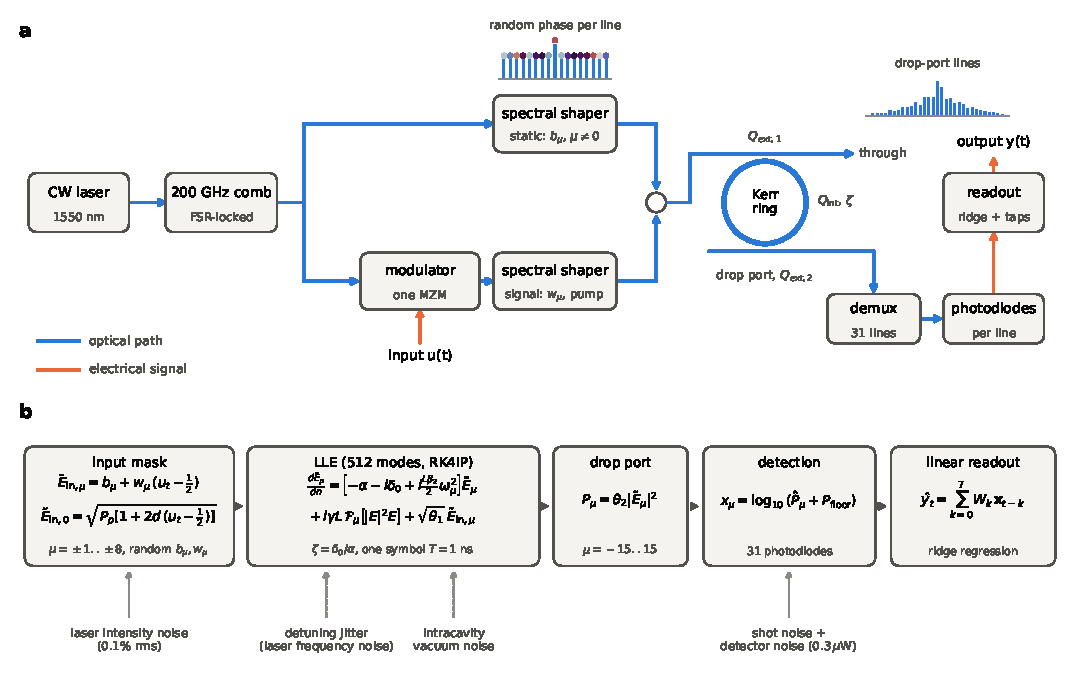
\includegraphics[width=\linewidth]{fig1_scheme}
\caption{方案与模型。
（a）光路：与微环自由光谱范围锁定的 $200~\mathrm{GHz}$ 输入光梳分成两路，静态的一路经谱整形器写入偏置 $b_\mu$ 并挡掉中心（泵浦）梳齿，
另一路经一个调制器承载信号 $u(t)$、再经谱整形器写入权重 $w_\mu$ 并放过泵浦，所以泵浦功率按式~\eqref{eq:mask} 被调制；
两路合束后送入加载--下载型 Kerr 微腔（输入耦合 $\Qone$、下载耦合 $\Qtwo$、本征 $\Qint$、归一化失谐 $\zeta$）。
下载端口的 31 根梳齿经解复用后分别探测，由带延迟抽头的岭回归读出层组合成输出 $y(t)$。插图：输入梳齿的随机相位（颜色）和下载端口光谱的示意。
（b）仿真模型的信号流：输入掩模（式~\eqref{eq:mask}）、Lugiato--Lefever 方程（式~\eqref{eq:lle}）、下载端口功率、对数探测和线性读出；
虚线箭头标出五项噪声进入的位置（第~\ref{sec:noise-model}~节）。}
\label{fig:scheme}
\end{figure}

腔内场用平均场的 Lugiato--Lefever 方程（LLE）描述~\cite{lugiato1987,coen2013}。
以往返次数 $n=t/t_R$ 为慢时间，记第 $\mu$ 个纵模（相对泵浦）的场振幅为 $\tilde E_\mu$，其角频率偏移为 $\omega_\mu=2\pi\,\mathrm{FSR}\,\mu$，则
\begin{equation}
\frac{\mathrm d\tilde E_\mu}{\mathrm dn}
=\Big[-\alpha-i\delta_0+i\frac{L\beta_2}{2}\,\omega_\mu^{2}\Big]\tilde E_\mu
+i\gamma L\,\mathcal F_\mu\!\big[|E|^{2}E\big]
+\sqrt{\theta_1}\,\tilde E_{\mathrm{in},\mu}(u_t),
\label{eq:lle}
\end{equation}
其中 $t_R=1/\mathrm{FSR}$ 是往返时间，$E(\tau)$ 是快时间网格上的腔内场（$|E|^2$ 以瓦为单位），$\mathcal F_\mu$ 表示取第 $\mu$ 个傅里叶分量
（约定 $E(\tau)=\sum_\mu\tilde E_\mu e^{-i\omega_\mu\tau}$），$\alpha_i$ 是每往返一次的本征功率损耗，
$\theta_1$、$\theta_2$ 是两个端口的功率耦合率，$\alpha=(\alpha_i+\theta_1+\theta_2)/2$ 是每往返一次的场衰减（半线宽），
$\delta_0$ 是泵浦相对谐振的失谐。下文用归一化失谐 $\zeta=\delta_0/\alpha$（以半线宽为单位）。
总品质因数与衰减的关系为 $Q=\omega_0 t_R/(2\alpha)$。
下载端口第 $\mu$ 根梳齿的光功率为 $P_\mu=\theta_2|\tilde E_\mu|^{2}$。

方程~\eqref{eq:lle} 用相互作用绘景下的四阶龙格--库塔法（RK4IP）~\cite{hult2007} 积分，只由快速傅里叶变换和逐点运算构成，
因此可以对所有器件参数求梯度（第~\ref{sec:gradient}~节）。
默认用 512 个纵模，每个 $1~\mathrm{ns}$ 的符号（约 200 次往返）积分 20 步。
我们检查了网格收敛：主结果在 512 与 1024 个模式之间一致，早先观察到的约 30\% 差别来自选点时的乐观偏差，而不是网格（补充材料）。

\subsection{输入编码}\label{sec:encodings-def}

输入信号是一串符号 $u_t\in[0,1]$，每个符号持续 $T=1~\mathrm{ns}$，期间输入场保持不变。
我们比较八种把 $u_t$ 送进微环的方式。

\paragraph{谱相位输入掩模（本文）。}
输入场由泵浦（$\mu=0$）和两侧各 8 根输入梳齿（$\mu=\pm1,\dots,\pm8$）组成：
\begin{equation}
\tilde E_{\mathrm{in},0}=\sqrt{P_p\,[1+2d\,(u_t-\tfrac12)]},\qquad
\tilde E_{\mathrm{in},\mu}=b_\mu+w_\mu\,(u_t-\tfrac12)\quad(\mu=\pm1,\dots,\pm8).
\label{eq:mask}
\end{equation}
每根梳齿的偏置 $b_\mu$ 和调制权重 $w_\mu$ 是独立抽取的复高斯数，即随机的幅度和随机的相位；
它们整体缩放，使边带的平均功率 $\sum_\mu\big(|b_\mu|^{2}+|w_\mu|^{2}/12\big)$ 等于总功率 $P$ 的一个比例 $f_s$，泵浦功率 $P_p=(1-f_s)P$。
每个工作点的随机参数是总功率 $P$（$10$ 到 $300~\mathrm{mW}$，对数均匀）、$f_s\in[0.1,0.9]$、调制深度 $d\in[0.05,0.9]$、$\zeta\in[-1,4]$ 和 $\Qone$。
在实验上，这相当于把一个输入光梳分成两路，一路保持静止（给出 $b_\mu$），一路经过一个调制器（给出 $w_\mu$），
两路各经过一个可编程的谱整形器后再合束。第~\ref{sec:ablation}~节的消融显示，真正起作用的是各梳齿相位的随机性，
所以谱整形器只需要设定相位。

\paragraph{单泵浦编码（我们对文献方案的实现）。}
只用一个连续泵浦，信号调制它的功率 $P[1+d(u_t-\tfrac12)]$、失谐 $\zeta+d(u_t-\tfrac12)$ 或相位 $\exp[i d(u_t-\tfrac12)]$，
分别参照文献~\cite{shishavan2025}、\cite{cuevas2025}、\cite{arabieh2026soliton}。这些是放在统一器件和协议下的实现，不是对原文装置的复现
（原文没有给全腔长、$Q$ 分配和采样间隔）。三种编码各有两组。从零场起振时，$\zeta\in[-1,4]$、$P\in[10,300]~\mathrm{mW}$ 与掩模相同，
功率编码 $d\in[0.05,1]$，失谐和相位编码的 $d$ 在 $[10^{-1.3},10^{0.5}]$ 内对数均匀抽取。
从单孤子出发时，$\Qone\in[10^{6.5},10^{7.2}]$、$P\in[30,300]~\mathrm{mW}$，$\zeta$ 在孤子存在区间内（从 2 到其上限）抽取，
功率编码 $d\in[0.02,0.5]$，失谐编码 $d$ 在 $[10^{-1.3},10^{0}]$、相位编码在 $[10^{-1.3},10^{0.5}]$ 内对数均匀抽取。

\paragraph{整体调制的光梳。}
与掩模相同的 16 根输入梳齿，但幅度相同、相位相同，所有梳齿一起被同一个信号调制，相当于一串被调制的同步脉冲~\cite{arabieh2026pulse}。

所有编码使用相同的器件、相同的功率和 $Q$ 范围、相同的读出，并且各抽相同数量的随机工作点（第~\ref{sec:protocol}~节）。

\subsection{读出}\label{sec:readout-def}

下载端口的中心 31 根梳齿（$\mu=-15,\dots,15$）经解复用后由光电探测器分别探测。
读数取对数，$x_\mu=\log_{10}(\hat P_\mu+P_\mathrm{floor})$，其中 $\hat P_\mu$ 是带噪声的读数，
$P_\mathrm{floor}$ 取探测器噪声与 $1~\mathrm{nW}$ 中较大者，避免没有光的梳齿在取对数后主导回归。
读出层除了当前符号的 31 个读数，还看前 7 个符号的读数（8 个延迟抽头，共 248 个特征；NARMA-10 用 12 个抽头），
用带标准化的岭回归，正则化强度在 $\{10^{-8},10^{-6},10^{-4},10^{-2},1\}$ 中按验证误差选取。
第~\ref{sec:memory}~节专门讨论这些抽头带来的记忆。

\subsection{噪声模型}\label{sec:noise-model}

“现实噪声”包括器件内的三项和探测端的两项：
\begin{itemize}
\item 激光强度噪声：相对均方根 $0.1\%$，每个符号一个样本，泵浦和所有输入梳齿共用；
\item 失谐抖动：泵浦相对谐振的失谐每个符号抖动半线宽的 $1\%$（均方根），为一阶自回归过程，相邻符号的相关系数为 $e^{-1}$。
      因为它按线宽的比例定义，等效的激光线宽随 $Q$ 变化（式~\eqref{eq:linewidth}）：$Q=1.9\times10^{6}$ 时约 $1.6~\mathrm{kHz}$，$Q=6\times10^{6}$ 时只有约 $160~\mathrm{Hz}$。
      所以随机搜索对高 $Q$ 点的惩罚比固定的激光轻；第~\ref{sec:laser}~节对最好的单环改用绝对的激光频率噪声谱，在固定激光下的全面重选留作后续工作；
\item 腔内场噪声：真空涨落水平，每个损耗通道每个模式半个光子；
\item 散粒噪声：每个读数积分一个符号时间（$1~\mathrm{ns}$）；
\item 探测器电子噪声：每根梳齿 $0.3~\mu\mathrm{W}$（折合到光功率的均方根）。
      1~GHz 量级的 InGaAs PIN 接收机，按手册的等效噪声功率折算为每根梳齿 $0.13$ 到 $0.63~\mu\mathrm{W}$，$0.3~\mu\mathrm{W}$ 居中。
\end{itemize}
放大器自发辐射的自拍频噪声和探测器量子效率没有建模。第~\ref{sec:noise}~节逐项拆分这些噪声的贡献。

\subsection{任务与软件基线}\label{sec:tasks}

三个基准任务：
（1）Mackey--Glass 时间序列~\cite{mackey1977}（延迟 17，反馈率 0.2、衰减率 0.1，指数 10，采样间隔 1）的 10 步预测；
（2）非线性信道均衡~\cite{jaeger2004}：四电平符号经过线性符号间干扰、三阶多项式非线性和信噪比 $28~\mathrm{dB}$ 的加性噪声，
从接收信号恢复两个符号之前发送的符号，除 NMSE 外还报告误符号率；
（3）NARMA-10~\cite{atiya2000}，它需要约 10 个符号的记忆。
补充材料另给出一个真实的光纤链路任务（28~GBd PAM-4、17~km 标准单模光纤、强度调制直接探测）。

软件基线有两个。一是回声状态网络（ESN）~\cite{jaeger2001}：31 个 $\tanh$ 节点，与微环的读出维度相同，
读出层看同样多的延迟抽头，谱半径（0.5 到 1.1）和输入尺度（0.1 到 1）在验证集上选。表~\ref{tab:encodings} 只用一个随机储备池；
第~\ref{sec:software}~节用 3 个随机储备池，并另给出 100 到 1000 个节点的 ESN 和下一代储备池计算（NG-RC）~\cite{gauthier2021}。
ESN 的搜索比微环小（12 组超参数，没有泄漏率和偏置，参见~\cite{lukosevicius2012}），不同随机储备池之间差别也不小：
输入噪声 $3\times10^{-3}$ 时，31 节点 ESN 用表~\ref{tab:encodings} 的单个储备池为 $3.2\times10^{-4}$，用第~\ref{sec:software}~节的 3 个储备池为 $1.9\times10^{-4}$，
结论依赖于它时两个数都给出。二是线性自回归，用最多 32 个滞后输入。
现实噪声下，基线的输入加上均方根 $3\times10^{-3}$ 的噪声，即把激光强度噪声按调制深度 $0.33$ 折算到输入；
这个约定对比较结论影响很大，第~\ref{sec:software}~节给出完整的扫描。

\subsection{评估协议}\label{sec:protocol}

每条序列先丢弃 300 个预热符号，再用 1700 个符号，按 60/20/20 分成训练、验证和测试三段
（信道均衡在现实噪声下另把测试段加长到 5000 个符号，以分辨误符号率）。
误差用归一化均方误差衡量，$\mathrm{NMSE}=\langle(\hat y_t-y_t)^2\rangle/\mathrm{var}(y_t)$，在测试段上计算。
一个物理器件不会两次遇到同样的噪声，因此读出层总是在一次运行上训练、在另一次噪声独立的运行上测试（跨运行 NMSE）。
同一输入驱动的两次运行 $a$、$b$ 的一致性定义为 31 根梳齿上（取对数、不加抽头的）特征相关系数的平均，
$C=\frac{1}{31}\sum_\mu\mathrm{corr}_t\big(x^{(a)}_{\mu,t},x^{(b)}_{\mu,t}\big)$，不变化的梳齿不计入~\cite{uchida2004}。

工作点的选择分两步，以免挑中只是碰巧运气好的点：
先对每种编码抽 256 个随机工作点，各跑一对运行，按验证误差取前 16 个；
再让这 16 个点各跑 3 对新的运行，选平均验证误差最小的一个；
最后报告它在另外 6 对新运行上的平均测试误差。每种设置做 3 条独立的序列，报告几何平均。
如果只按一次噪声实现挑选并报告，结果会乐观 10\% 到 30\%（补充材料）。

\section{相干种子区：为什么输出可以重复}\label{sec:mechanism}

储备池计算要求同样的输入给出同样的输出，即一致性或回声状态性质~\cite{jaeger2001,uchida2004}，否则训练好的读出层换一次运行就失效。
文献中的单泵浦方案里，梳齿要么由调制不稳定性从噪声中长出来~\cite{shishavan2025}，要么依赖预先建立的孤子态~\cite{cuevas2025,arabieh2026soliton}。
前者的输出取决于起振时的噪声，后者需要把器件稳定在孤子存在区间内。
用谱相位掩模时，输入梳齿本身就落在谐振上，其余梳齿由它们经四波混频产生，是由输入相干地“种”下去的，而不是从噪声中长出来，
这与脉冲或光梳驱动的 Kerr 腔类似~\cite{obrzud2017}。

\subsection{两次运行的比较}

图~\ref{fig:two-runs} 把同一个输入序列送进同一个器件两次，两次运行只有初始的腔内噪声不同。
（a）是原始混沌光梳方案的参数（单个连续泵浦，$325~\mathrm{mW}$，总品质因数 $10^{7}$，归一化失谐约 5；这个点在我们随机搜索的失谐范围之外，见第~\ref{sec:encodings-def}~节）：
由调制不稳定性产生的第 3 根梳齿在两次运行中完全不同，相关系数只有 $0.08$，用这样的特征训练读出层，换一次运行后 NMSE 约为 1。
（b）（c）是一个谱相位掩模的工作点（第~\ref{sec:noise}~节噪声下限研究中选出的点，$23~\mathrm{mW}$，总品质因数 $6\times10^{6}$）。
对输入梳齿（$\mu=3$，图 b），两次重合是意料之中的，因为它被直接驱动；真正的检验是只靠四波混频产生的梳齿（$\mu=12$，图 c，在输入梳齿 $|\mu|\le8$ 之外）。
它的两次运行同样重合，相关系数为 $1.00$，功率比输入梳齿低约十倍。

\begin{figure}[htbp]
\centering
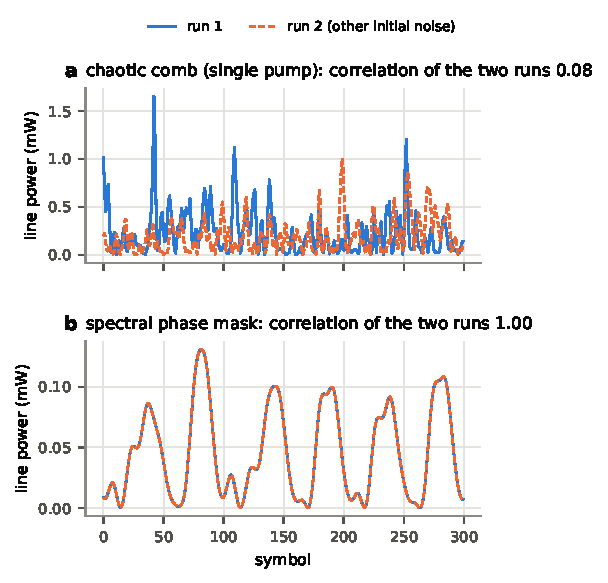
\includegraphics[width=0.8\linewidth]{fig3_two_runs}
\caption{同一输入序列送入同一器件两次，两次运行只有初始的腔内噪声不同（实线和虚线），画出下载端口的梳齿功率（前 300 个符号，不加其他噪声）。
（a）原始混沌光梳方案的参数（单个连续泵浦，$325~\mathrm{mW}$，总品质因数 $10^{7}$，归一化失谐约 5），产生的梳齿 $\mu=3$：相关系数 $0.08$。
（b）（c）谱相位掩模的一个工作点（$23~\mathrm{mW}$，总品质因数 $6\times10^{6}$）：（b）输入梳齿 $\mu=3$，（c）只靠四波混频产生的梳齿 $\mu=12$；相关系数都是 $1.00$。注意纵轴量级不同。}
\label{fig:two-runs}
\end{figure}

\subsection{工作区图}

可重复性只在一定的参数范围内成立。图~\ref{fig:operating-map} 以表~\ref{tab:encodings} 中现实噪声下 Mackey--Glass 选出的掩模工作点为中心，
保持其失谐、调制深度、功率分配和掩模不变，只扫描输入耦合品质因数 $\Qone$（$10^{5.6}$ 到 $10^{7.6}$）和总输入功率（$3$ 到 $1000~\mathrm{mW}$），各取 17 档。
每个格点只用一条序列、一对运行评估，所以是单次噪声实现的值（图中最好的误差 $1.8\times10^{-6}$ 和 $3.3\times10^{-4}$ 恰好舍入后与表~\ref{tab:encodings} 相同）。

无噪声时，74\% 的点一致性高于 $0.99$，是相干种子区。不一致的点（一致性低于 $0.5$，占 16\%）在图~\ref{fig:operating-map}a 实线等值线之外，处于高功率、高 $Q$ 区
（最高 $Q$ 处约 $150~\mathrm{mW}$ 以上，$\Qone\approx2\times10^{6}$ 处约 $1~\mathrm{W}$ 以上），那里调制不稳定性压过输入的种子，光梳回到混沌。
误差在失去一致性之前就已经升高（两条等值线之间），所以高误差和不一致不是一回事。
误差最小的区域在相干种子区内部、靠近混沌区的一侧：误差在最好值 3 倍以内的点都落在 $6$ 到 $79~\mathrm{mW}$、$\Qone=10^{6.1}$ 到 $10^{6.85}$ 之间，
符合“非线性越强越有用，直到失去可重复性”的一般经验。

现实噪声下多出第三个区域。功率太低时，许多梳齿到达探测器的光与探测器噪声相当，读数被淹没，一致性同样下降（图~\ref{fig:operating-map}b 下方虚线以下）；
一致性高于 $0.99$ 的点从 74\% 降到 29\%。可用的点被夹在两者之间：误差在最好值 3 倍以内的点在功率--$Q$ 平面上连成一条斜带（$9$ 到 $336~\mathrm{mW}$），
随 $Q$ 升高向低功率方向倾斜，因为 $Q$ 越高，产生同样非线性所需的功率越低。混沌区在有噪声和无噪声时位置基本相同，因为它的成因（调制不稳定性的增益超过输入种子）与噪声无关。

\begin{figure}[htbp]
\centering
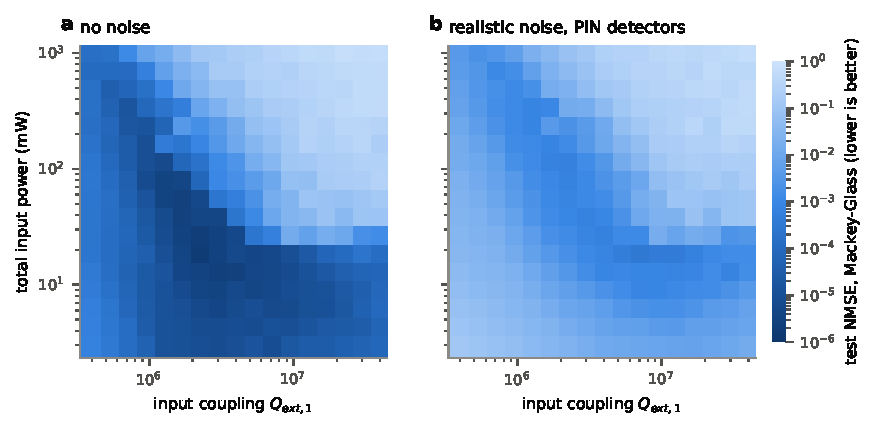
\includegraphics[width=\linewidth]{fig2_operating_map}
\caption{谱相位掩模在表~\ref{tab:encodings} 工作点附近的工作区图（Mackey--Glass，一条序列，每个格点一对运行）。固定其余参数，扫描输入耦合品质因数 $\Qone$ 和总输入功率（各 17 档），
颜色为测试误差（越深越好）。虚线和实线：两次运行一致性为 $0.99$ 和 $0.5$ 的等值线；星号：误差最小点。
（a）无噪声：实线之外（高功率、高 $Q$）是不可重复的混沌区。（b）现实噪声、PIN 探测器：下方虚线以下读数被探测器噪声淹没，可用点在两区之间连成一条带。}
\label{fig:operating-map}
\end{figure}

这一节的结论在后面反复用到：谱相位掩模工作在相干种子、可重复的区域，它的误差来自噪声，而不是不可重复的动力学。
去掉 Kerr 项的对照（第~\ref{sec:linear}~节）表明，掩模在 Mackey--Glass 上的好处主要来自 Kerr 动力学，在信道均衡上则不是：
那里相互干涉的输入梳齿经平方律探测就已提供所需的非线性。

\section{编码对比}\label{sec:encodings}

本节在完全相同的物理条件下比较八种编码：同一个仿真器、同样的器件参数范围和光功率范围、同样的读出（31 根梳齿、8 个抽头）、
同样的噪声模型，以及同样数量的随机工作点和同样的选点流程（第~\ref{sec:protocol}~节）。
表~\ref{tab:encodings} 汇总了三个任务在无噪声和现实噪声下的结果，图~\ref{fig:encodings} 画出同样的数字。

% generated by experiments/make_table1.py; do not edit by hand
\begin{table}[htbp]
\centering
\caption{各编码与基线的测试误差（NMSE，越小越好）。每种编码在相同范围内各抽 256 个随机工作点，按新运行的平均验证误差选点，报告另外 6 组新运行的平均测试误差，再取 3 条序列的几何平均；读出层训练在一次运行上、测试在另一次噪声独立的运行上。每列最好的微环编码用粗体标出。ESN 与微环的读出维度相同（31 个节点、相同的延迟抽头），只用一个随机储备池，现实噪声下给它的输入噪声为 $3\times10^{-3}$；更强的软件基线见第~\ref{sec:software}~节。信道均衡在现实噪声下的测试段为 5000 个符号。}
\label{tab:encodings}
\small
\begin{tabular}{lcccccc}
\toprule
 & \multicolumn{2}{c}{Mackey--Glass（10 步预测）} & \multicolumn{2}{c}{非线性信道均衡} & \multicolumn{2}{c}{NARMA-10} \\
\cmidrule(lr){2-3}\cmidrule(lr){4-5}\cmidrule(lr){6-7}
编码 & 无噪声 & 现实噪声 & 无噪声 & 现实噪声 & 无噪声 & 现实噪声 \\
\midrule
泵浦功率~\cite{shishavan2025} & $0.20$ & $0.33$ & $7.6\times10^{-3}$ & $1.0\times10^{-2}$ & $0.21$ & $0.35$ \\
泵浦失谐~\cite{cuevas2025} & $5.6\times10^{-2}$ & $9.3\times10^{-2}$ & $1.2\times10^{-2}$ & $3.0\times10^{-2}$ & $0.21$ & $0.45$ \\
泵浦相位~\cite{arabieh2026soliton} & $0.14$ & $0.20$ & $4.8\times10^{-2}$ & $7.7\times10^{-2}$ & $0.66$ & $1.0$ \\
泵浦功率，孤子起点 & $1.9\times10^{-3}$ & $5.3\times10^{-2}$ & $1.1\times10^{-2}$ & $2.1\times10^{-2}$ & $0.20$ & $0.32$ \\
泵浦失谐，孤子起点 & $1.7\times10^{-3}$ & $9.5\times10^{-2}$ & $1.2\times10^{-2}$ & $0.17$ & $0.19$ & $0.39$ \\
泵浦相位，孤子起点 & $2.8\times10^{-3}$ & $5.0\times10^{-2}$ & $3.5\times10^{-2}$ & $6.0\times10^{-2}$ & $0.68$ & $0.74$ \\
整体调制光梳 & $8.2\times10^{-5}$ & $4.8\times10^{-3}$ & $5.0\times10^{-3}$ & $7.6\times10^{-3}$ & $0.18$ & $0.21$ \\
谱相位掩模（本文） & $\mathbf{1.8\times10^{-6}}$ & $\mathbf{3.3\times10^{-4}}$ & $\mathbf{3.7\times10^{-3}}$ & $\mathbf{5.7\times10^{-3}}$ & $\mathbf{0.16}$ & $\mathbf{0.19}$ \\
\midrule
ESN（31 节点） & $2.4\times10^{-5}$ & $3.2\times10^{-4}$ & $3.8\times10^{-3}$ & $4.0\times10^{-3}$ & $0.11$ & $0.11$ \\
线性自回归 & $0.14$ & $0.21$ & $1.1\times10^{-2}$ & $1.3\times10^{-2}$ & $0.19$ & $0.19$ \\
\bottomrule
\end{tabular}
\end{table}


\begin{figure}[htbp]
\centering
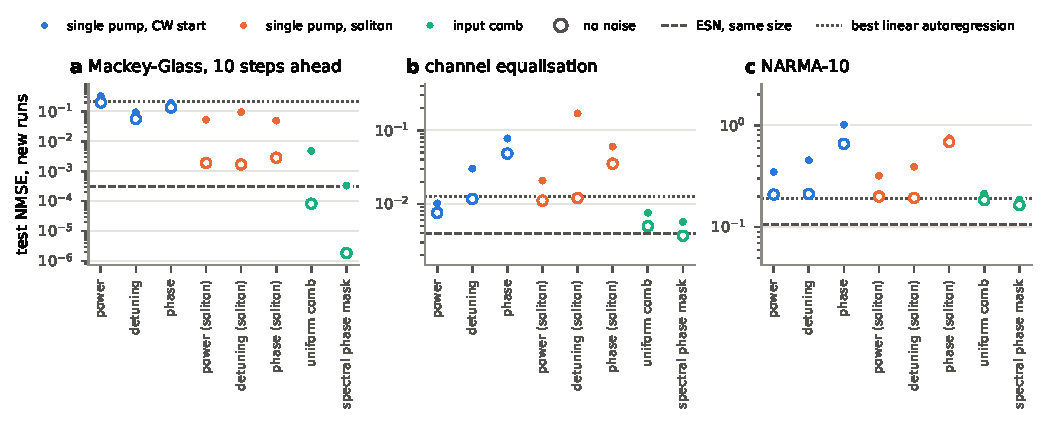
\includegraphics[width=\linewidth]{fig4_encodings}
\caption{现实噪声下八种编码在三个任务上的测试误差（表~\ref{tab:encodings} 的“现实噪声”列；新运行复测，3 条序列的几何平均）。
蓝色：从零场起振的单泵浦编码；橙色：从单孤子出发的单泵浦编码；绿色：输入光梳（整体调制和谱相位掩模）。
虚线为同读出维度的 ESN（输入噪声 $3\times10^{-3}$），点线为最好的线性自回归。
（a）Mackey--Glass 10 步预测；（b）非线性信道均衡；（c）NARMA-10。}
\label{fig:encodings}
\end{figure}

\subsection{Mackey--Glass 预测}

谱相位掩模在 Mackey--Glass 上的优势最大。无噪声时它的测试误差为 $1.8\times10^{-6}$，
比整体调制的光梳（$8.2\times10^{-5}$）好约 45 倍，比最好的单泵浦编码（从孤子出发的失谐编码，$1.7\times10^{-3}$）好约 900 倍，
比从零场起振的单泵浦编码好四到五个数量级。
现实噪声下所有编码都变差，但次序不变：掩模为 $3.3\times10^{-4}$，整体调制的光梳为 $4.8\times10^{-3}$（差约 15 倍），
最好的单泵浦编码为 $5.0\times10^{-2}$（差约 150 倍）。

同读出维度的 ESN 在无噪声时为 $2.4\times10^{-5}$，掩模比它好约 13 倍；
现实噪声下 ESN 为 $3.2\times10^{-4}$，与掩模持平。
后一个比较依赖于给 ESN 设定的输入噪声：这里用的是 $3\times10^{-3}$，而且 ESN 只用了一个随机储备池；
多试几个储备池后 ESN 降到 $1.9\times10^{-4}$，输入噪声降到 $10^{-3}$ 时更降到 $5.3\times10^{-5}$。
第~\ref{sec:software}~节专门讨论这种比较，本节只比较光学编码之间的差别，它们共享同一套噪声模型，不受这个约定影响。

\subsection{优势不是来自单个幸运的工作点}

一种编码的最好结果，可能只是在 256 次随机抽取中碰上了一个特别好的点。
图~\ref{fig:distributions} 给出每种编码全部随机工作点的误差分布（现实噪声下的 Mackey--Glass，3 条序列共 768 个点）。
掩模的整个分布都明显左移：它的中位数为 $4.3\times10^{-2}$，已经好于每一种单泵浦编码最好的那 10\% 的点（$0.14$ 到 $0.38$）；
最好的 10\% 掩模工作点低于 $1.9\times10^{-3}$，比整体调制光梳最好的 10\%（$2.5\times10^{-2}$）好一个数量级以上。
所以掩模的优势是这一类输入方式整体的性质，不依赖于某个特别的参数组合。

\begin{figure}[htbp]
\centering
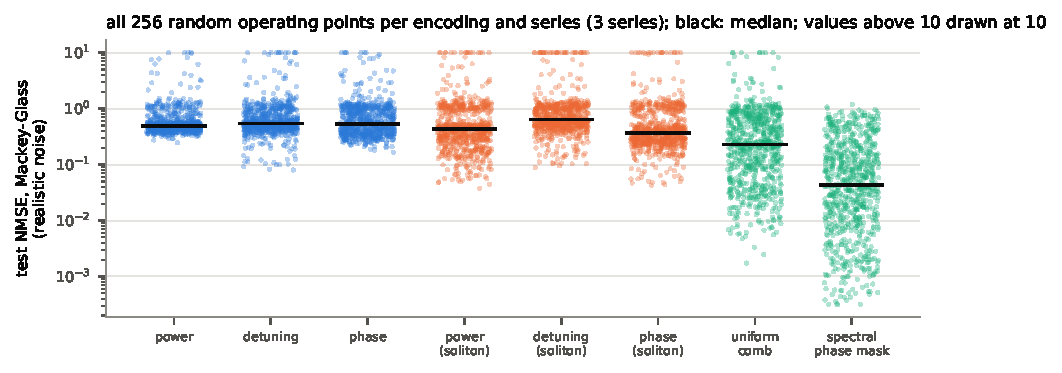
\includegraphics[width=\linewidth]{fig5_distributions}
\caption{现实噪声下 Mackey--Glass 的测试误差分布：每种编码每条序列 256 个随机工作点（3 条序列共 768 个点，每点一对运行），黑线为中位数；
高于 10 的值画在 10 处。颜色与图~\ref{fig:encodings} 相同。}
\label{fig:distributions}
\end{figure}

\subsection{信道均衡}

信道均衡上的差别小得多。掩模仍是最好的光学编码，无噪声时为 $3.7\times10^{-3}$，现实噪声下为 $5.7\times10^{-3}$，
比整体调制的光梳好约 1.3 倍，比最好的单泵浦编码（功率编码）好约 2 倍，比线性自回归（$1.1\times10^{-2}$ 和 $1.3\times10^{-2}$）好 2 到 3 倍。
无噪声时掩模与 ESN（$3.8\times10^{-3}$）持平；现实噪声下 ESN 为 $4.0\times10^{-3}$，比掩模好约 1.4 倍。
这个任务的误差主要来自信道本身的噪声，第~\ref{sec:software}~节显示，把 ESN 的输入噪声降到零它也只改善约 7\%。
按误符号率看（每条序列 6 组新运行、每组 5000 个测试符号，3 条序列共 9 万个符号），掩模为 $1.9\times10^{-4}$（17 个错误），
整体调制的光梳为 $1.0\times10^{-4}$（9 个），功率编码为 $3.9\times10^{-4}$（35 个），ESN 为 $1.1\times10^{-5}$（1 个）。
掩模与整体调制的光梳在这个统计量下分不开；所有光梳编码和 ESN 都远低于常用的硬判决纠错门限 $3.8\times10^{-3}$。

\subsection{NARMA-10：单环不成立的例子}

NARMA-10 需要约 10 个符号的记忆，而微环自身的记忆只有光子寿命，几个符号以内。
单个微环上，掩模（无噪声 $0.16$，现实噪声 $0.19$）只与线性自回归（$0.19$）持平，略好于整体调制的光梳和单泵浦编码，
但比 ESN（$0.11$）差约 1.5 到 1.8 倍。我们把它作为不成立的例子如实报告。
记忆可以从外部补上：给输入梳齿再加一份延迟后的信号（输入延迟线），并把几个掩模不同的环拼接读出后，
NARMA-10 降到 $0.011$，与带同样延迟线的 100 节点 ESN（$0.010$）持平（第~\ref{sec:memory}~节和补充材料）。

\subsection{起作用的是梳齿相位的随机性}\label{sec:ablation}

为了弄清掩模的哪一部分在起作用，我们在相同的工作点范围内比较了几种简化的掩模（现实噪声，与表~\ref{tab:encodings} 相同的流程；补充图 S1）。
在 Mackey--Glass 上：
\begin{itemize}
\item 只让相位随机、所有梳齿幅度相同的掩模为 $2.4\times10^{-4}$，与完整掩模（这组运行中为 $3.8\times10^{-4}$）一样好或略好；
\item 只让幅度随机、所有梳齿同相的掩模为 $1.3\times10^{-3}$，差 3 到 6 倍；
\item 随机的静态光谱加一个统一的调制（$w_\mu\propto b_\mu$）为 $6.5\times10^{-4}$；
\item 幅度和相位都相同的整体调制为 $5.0\times10^{-3}$。
\end{itemize}
信道均衡上的次序相同（只调相位 $5.0\times10^{-3}$，完整掩模 $5.4\times10^{-3}$，只调幅度 $5.8\times10^{-3}$，整体调制 $7.3\times10^{-3}$），只是差别更小。
输入梳齿的数量也有影响：Mackey--Glass 上 4、8、16、32、64 根分别为
$1.9\times10^{-3}$、$1.4\times10^{-3}$、$3.8\times10^{-4}$、$2.4\times10^{-4}$、$2.1\times10^{-4}$，32 根以后不再明显改善；
信道均衡上 32 根最好（$4.0\times10^{-3}$），64 根反而变差（$5.6\times10^{-3}$）。

这给出第一条设计规则：\emph{起作用的是各梳齿相位的随机性，而不是每根梳齿独立的幅度调制}。
实现上不需要逐梳齿的调制器，一个调制器加两个只设相位的谱整形器就够了。
为什么相位比幅度重要，我们还没有完整的解释。一个直观的猜想是：随机相位让不同梳齿经四波混频进入同一根输出梳齿的各条路径以不同方式干涉，
使各输出梳齿的特征彼此更不相关。但这个猜想在线性层面上不成立。我们在每种变体选出的工作点上（无噪声，Mackey--Glass）计算了 31 路特征的相关矩阵：
有效秩（参与率，特征值之和的平方除以特征值平方之和）在整体调制、随机谱加统一调制、只调幅度、只调相位和完整掩模之间分别为
$2.2$、$2.3$、$2.4$、$2.2$、$2.0$，平均相关系数的绝对值为 $0.58$、$0.58$、$0.57$、$0.60$、$0.65$，几种变体几乎相同，完整掩模的线性多样性甚至最低。
所以掩模的好处不在于瞬时特征之间的线性去相关，而更可能在于各特征是输入历史的不同的高阶非线性函数；这需要用信息处理容量一类的分解来检验，留作后续工作。

\section{噪声下限}\label{sec:noise}

现实噪声让谱相位掩模在 Mackey--Glass 上的误差从 $1.8\times10^{-6}$ 升到 $3.3\times10^{-4}$，差约 180 倍（表~\ref{tab:encodings}）。
第~\ref{sec:mechanism}~节说明，掩模工作在相干种子区，误差来自噪声而不是不可重复的动力学。
本节把五项噪声拆开，回答三个问题：下限由哪几项决定；换用非线性更强的材料、加功率能不能降低它；它能不能在读出端扣除。
结论是：下限约一半来自失谐抖动、一半来自散粒噪声；前一半与光子数无关；后一半虽然随光子数下降，但光子一多，前一半就成为主导，所以换 Si$_3$N$_4$ 和加功率都几乎无效；
把真实的抖动序列交给线性读出层只能去掉 2\% 的误差，所以抖动只能在光源处压低，这给出对激光线宽的要求。

\subsection{逐项拆分}\label{sec:breakdown}

为了把探测器的影响和器件内部的噪声分开，先假设探测器是理想的（没有电子噪声，只有散粒噪声），在 256 个随机工作点中按第~\ref{sec:protocol}~节的流程选出最优点，
再在这个点上一次只打开一项噪声（图~\ref{fig:noise}a）。
这个点的总功率为 $23~\mathrm{mW}$，总品质因数 $6\times10^{6}$，每根梳齿到达探测器约 $170~\mu\mathrm{W}$，即每个符号约 $1.3\times10^{6}$ 个光子。
它无噪声时的误差为 $1.3\times10^{-5}$。只打开激光强度噪声时为 $1.9\times10^{-5}$，几乎不变；
只打开腔内真空噪声时为 $2.5\times10^{-5}$；只打开失谐抖动时为 $5.7\times10^{-5}$；只打开散粒噪声时为 $6.8\times10^{-5}$。
三项光学噪声一起为 $7.8\times10^{-5}$，再加上散粒噪声为 $1.5\times10^{-4}$。
所以理想探测器下的误差下限约为 $1.3\times10^{-4}$（256 个点重新选点后的值），其中约一半来自失谐抖动，一半来自散粒噪声，
腔内真空噪声次要，激光强度噪声可以忽略。

换成现实的 PIN 探测器（每根梳齿 $0.3~\mu\mathrm{W}$ 的电子噪声），同样流程选出的最优点为 $3.4\times10^{-4}$，又差约 2.5 倍。
探测器噪声的影响在一个较早、较小规模的搜索（每种编码 32 个候选点，单次运行选点）中看得最清楚：
全部噪声打开、探测器噪声为 $0.03$、$0.1$、$0.3$、$0.6~\mu\mathrm{W}$ 时，误差为
$2.7\times10^{-4}$、$4.1\times10^{-4}$、$1.0\times10^{-3}$、$2.2\times10^{-3}$，在 $0.1~\mu\mathrm{W}$ 以上近似随探测器噪声线性增长；
在 $0.3~\mu\mathrm{W}$ 的探测器前加一级增益 $10~\mathrm{dB}$ 或 $20~\mathrm{dB}$、噪声系数 $5~\mathrm{dB}$ 的光放大器，误差降到 $3.3\times10^{-4}$ 和 $3.1\times10^{-4}$，
接近只有光学噪声和散粒噪声时的 $2.4\times10^{-4}$。
这个搜索的绝对数值与表~\ref{tab:encodings} 不能直接比（候选点少、选点方式不同），这里只用它看趋势：
探测器电子噪声是可以用光放大器去掉的一项，去掉之后剩下的就是上面的下限。

\begin{figure}[htbp]
\centering
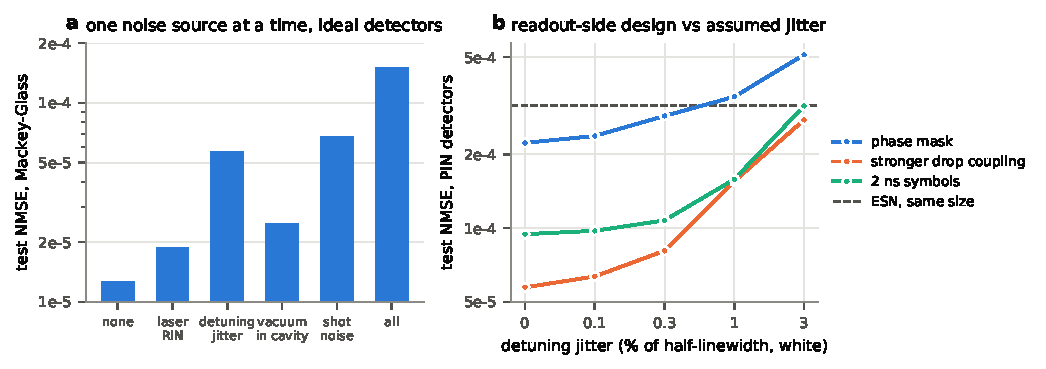
\includegraphics[width=\linewidth]{fig6_noise}
\caption{噪声与读出侧设计（Mackey--Glass）。
（a）理想探测器下，在 256 个点中选出的最优工作点上一次只打开一项噪声时的测试误差；“all”为四项（激光强度噪声、失谐抖动、腔内真空噪声、散粒噪声）同时打开；点线为同一点无噪声时的值。(a)(b) 中各点均为 3 条序列、每条 6 对新运行的几何平均。
（b）每档抖动重新选点后的测试误差随所假设的失谐抖动（每符号均方根，以半线宽的百分比计，相邻符号相关系数 $e^{-1}$；横轴为类别轴）的变化，PIN 探测器：
普通的谱相位掩模、加大下载端口耦合、$2~\mathrm{ns}$ 符号；虚线为同读出维度的 ESN（输入噪声 $3\times10^{-3}$，一个随机储备池）。
上方横轴是加大下载端口耦合工作点（$Q=1.9\times10^{6}$，$1~\mathrm{ns}$）上产生同样抖动的激光本征线宽（式~\eqref{eq:linewidth}）；$2~\mathrm{ns}$ 符号的工作点（$Q=5\times10^{6}$）约为其 0.3 倍。}
\label{fig:noise}
\end{figure}

\subsection{换非线性更强的材料、加功率都动不了下限}\label{sec:platform}

散粒噪声带来的误差可以靠更多光子来降低，失谐抖动则不能：抖动是相对于谐振线宽定义的，与腔内有多少光子无关。
我们用两种方式增加或减少光子数，并在每种情况下重新搜索 256 个工作点（理想探测器）：
\begin{itemize}
\item 换成 Si$_3$N$_4$ 微环（非线性系数约为石英的 60 倍，功率范围按 $\gamma L$ 的比例缩小，使归一化泵浦覆盖同样的范围）：
      最优点只需 $5~\mathrm{mW}$，到达探测器的光子少了约 8 倍，但误差下限为 $1.4\times10^{-4}$，与石英的 $1.3\times10^{-4}$ 相同；
\item 石英微环，功率范围提高到 10 倍（$0.1$ 到 $3~\mathrm{W}$）：误差下限为 $1.5\times10^{-4}$，没有改善。
      在它的最优点，每根梳齿的光子数是上面那个点的 4.4 倍，但散粒噪声那一项只从 $6.8\times10^{-5}$ 降到 $5.3\times10^{-5}$，
      失谐抖动那一项（$5.1\times10^{-5}$）则基本不变。
\end{itemize}
散粒噪声那一项的下降远慢于光子数的增加，但这两个最优点的其他参数也不同，所以这只是一个粗略的比较。
一个受控的比较是固定工作点和腔内动力学，只改变每个读数探测到的光子数（最好的单环，理想探测器，3 条序列 $\times$ 6 对新运行）：
光子数为原来的 1、10、100 倍时，总误差为 $1.41\times10^{-4}$、$1.21\times10^{-4}$、$1.16\times10^{-4}$，
没有散粒噪声时为 $1.16\times10^{-4}$。散粒噪声那一项本身随光子数下降（10 倍光子降约 5 倍，100 倍降约 40 倍），
但总误差很快停在光学噪声（主要是失谐抖动）决定的水平上。在这个工作点上，加功率最多只能把误差降低约 18\%。
换 Si$_3$N$_4$ 的好处在功率：同样的下限只需约 1/4 的功率；但在普通探测器下，到达探测器的光少了，误差反而升到 $1.1\times10^{-3}$，
要配更好的探测器或光放大器才能用上。
能降低下限的是读出一侧：加大下载端口耦合（让更多光到达探测器）或把符号放慢到 $2~\mathrm{ns}$（每个读数积分更久），
理想探测器下分别降到 $8.7\times10^{-5}$ 和 $6.9\times10^{-5}$，普通探测器下为 $1.55\times10^{-4}$ 和 $1.58\times10^{-4}$（第~\ref{sec:readout}~节）。

\subsection{知道真实抖动的线性读出层也没有去掉它}\label{sec:reference}

如果失谐抖动主要来自泵浦激光的频率噪声，那么同一芯片上、由同一台激光驱动的所有微环都看到同样的抖动。
一个自然的想法是加一个不加信号的参考环，测出这部分共模噪声，让读出层把它减掉。
我们先测这个想法的上限：在最好的单环（加大下载端口耦合组，$Q=1.9\times10^{6}$，$178~\mathrm{mW}$）上，
直接把每次运行真实的抖动序列（当前和前 7 个符号）交给读出层，相当于一个没有噪声的理想参考。
3 条序列、每条 6 对新运行的结果是：原样读出为 $1.60\times10^{-4}$；加上真实抖动序列后为 $1.58\times10^{-4}$，只降 2\%；
再加上当前抖动与各梳齿特征的乘积项（让修正量可以随状态变化），反而略差，为 $1.65\times10^{-4}$。
而把抖动本身关掉、其余噪声不变时，误差降到 $5.7\times10^{-5}$，好 2.8 倍。

也就是说，抖动确实是下限的大头，但即使完全知道它，我们试过的线性读出也只去掉 2\% 的误差。
可能的原因是抖动不是叠加在读数上的加性噪声：它改变了腔内的失谐，经过非线性动力学改变了整个梳的状态，而且这个影响会延续到后面几个符号；
它对每根梳齿的作用取决于当时的状态，线性读出层去不掉它。
所以用线性读出的共参考环不成立。我们没有把参考环自己的 31 路梳齿特征（它们是抖动历史的非线性函数）交给读出层。
对梳齿特征取二次项的读出层（第~\ref{sec:nonlin-readout}~节）对有、无抖动的误差同样降低，抖动损失仍为 2.7；最直接的办法还是在物理上压低抖动。

\subsection{没有找到对抖动不敏感的工作点}\label{sec:sweetspot}

在谐振峰顶，透射功率对失谐是驻点，抖动只能以二阶形式进来。Kerr 频移和色散使这一点不可能对每个输入、每根梳齿同时成立，但也许存在一片敏感性较低的区域。
我们在最好的单环周围扫了 78 个点（归一化失谐 $-1$ 到 $4$、步长 $0.2$；功率为原来的 0.5、1、1.5 倍），每个点在 3 条序列上各用 3 对新运行，分别测有、无抖动的误差。
抖动损失接近 1 的点确实存在，但那里无抖动时的误差就有 $3\times10^{-3}$ 到 $2\times10^{-2}$；无抖动误差低于 $2\times10^{-4}$ 的 10 个点，抖动损失都在 1.4 到 3.5 之间，
在全部点上两者呈负相关（对数的相关系数为 $-0.66$）。有抖动时最好的点为 $1.28\times10^{-4}$，不比原工作点好。

可能的原因是信号和抖动走同一条通道。掩模调制腔内功率，主要通过 Kerr 频移改变有效失谐来作用于整个梳；抖动改变的也是这个失谐。
微环在某点算得好，正是因为它在那里对失谐响应强，因而对抖动也敏感。这与线性和二次读出都分不开两者的结果一致，
也促使我们把信号送进另一组共享抖动、但信号符号相反的模式（第~\ref{sec:bidir}~节）。

\subsection{激光本征线宽的要求}\label{sec:laser}

上面的噪声模型给每个符号一个均方根为半线宽 1\% 的失谐抖动。现在把它和激光联系起来。
设激光的频率噪声是白噪声，对应洛伦兹线宽 $\Delta\nu$（单边频率噪声谱 $S_\nu=\Delta\nu/\pi$），
则在一个符号时间 $T$ 内平均后的频率起伏方差为 $\Delta\nu/(2\pi T)$。
以谐振的半线宽 $\nu_0/(2Q)$ 为单位，每个符号的相对抖动 $\varepsilon$ 与线宽的关系为
\begin{equation}
\Delta\nu=2\pi T\left(\frac{\varepsilon\,\nu_0}{2Q}\right)^{2}.
\label{eq:linewidth}
\end{equation}
对最好的单环（$Q=1.9\times10^{6}$，半线宽 $51~\mathrm{MHz}$，$T=1~\mathrm{ns}$），1\% 的抖动对应约 $1.6~\mathrm{kHz}$ 的本征线宽，
0.3\% 和 0.1\% 分别对应约 $150~\mathrm{Hz}$ 和 $16~\mathrm{Hz}$；反过来，本征线宽 $100~\mathrm{kHz}$ 的激光会带来约 8\% 的抖动。
所需线宽随 $Q$ 的平方变严，随符号时间变松：第~\ref{sec:readout}~节 $2~\mathrm{ns}$ 符号的工作点 $Q=5\times10^{6}$，1\% 对应约 $470~\mathrm{Hz}$。

为了检验这个换算，我们直接按真实激光的频率噪声谱生成抖动：$S_\nu(f)=h_0+h_{-1}/f$，
其中 $h_0=\Delta\nu/\pi$ 是白频率噪声，$h_{-1}/f$ 是闪烁噪声（半导体激光的转折频率通常在 $1~\mathrm{MHz}$ 左右）；
激光被锁在谐振上，锁定环路对频率噪声的抑制用一个一阶高通 $f^{2}/(f^{2}+B^{2})$ 表示。
时间序列由频谱合成，在每个符号内平均，再除以半线宽，作为每次运行的失谐抖动；其余噪声不变。
表~\ref{tab:laser} 给出结果。

% generated by experiments/make_table2.py; do not edit by hand
\begin{table}[htbp]
\centering
\caption{真实激光下最好的单环（加大下载端口耦合组，Mackey--Glass，现实噪声的其余各项不变）。失谐抖动由激光的白频率噪声按每个符号平均得到；“固定工作点”是 1\% 抖动假设下选出的点（$Q=1.9\times10^{6}$），“重选”是在该激光的噪声下按第~\ref{sec:protocol}~节的流程重新选点（每条序列 56 个按 $Q$ 分档的候选）。3 条序列 $\times$ 6 对新运行。两列用了不同的噪声实现，同一个工作点在两列之间约有 9\% 的差别。}
\label{tab:laser}
\small
\begin{tabular}{p{4.2cm}cccc}
\toprule
激光本征线宽 & 每符号抖动 & 固定工作点 & 重选后 & 重选点的 $Q$ \\
\midrule
100~Hz & 0.25\% & $6.7\times10^{-5}$ & -- & -- \\
1.6~kHz & 1.00\% & $1.3\times10^{-4}$ & $1.2\times10^{-4}$ & $1.9\times10^{6}$ \\
16~kHz & 3.15\% & $3.1\times10^{-4}$ & $2.9\times10^{-4}$ & $1.9\times10^{6}$ \\
100~kHz & 7.88\% & $8.1\times10^{-4}$ & $6.4\times10^{-4}$ & $1.9\times10^{6}$、$2.5\times10^{6}$ \\
1~MHz & 24.92\% & $5.2\times10^{-3}$ & $1.6\times10^{-3}$ & $1.2\times10^{6}$ \\
\midrule
100~kHz，加闪烁噪声（转折 1~MHz）和 1~MHz 锁定 & 7.92\% & $8.3\times10^{-4}$ & -- & -- \\
1.6~kHz，加闪烁噪声（转折 10~MHz），不锁定 & 1.10\% & $1.8\times10^{-4}$ & -- & -- \\
\bottomrule
\end{tabular}
\end{table}


表~\ref{tab:laser} 给出四点。
第一，在纳秒符号下起决定作用的是本征（白噪声）线宽：一个 $1~\mathrm{ns}$ 符号对应约 $500~\mathrm{MHz}$ 的带宽，几乎全被白频率噪声占据，
而闪烁噪声的功率集中在低频；加入转折频率 $1~\mathrm{MHz}$ 的闪烁噪声和 $1~\mathrm{MHz}$ 的锁定后，$100~\mathrm{kHz}$ 那一行几乎不变；
只有闪烁噪声极强（转折 $10~\mathrm{MHz}$）且完全不锁定时，$1.6~\mathrm{kHz}$ 那一行才从 $1.3\times10^{-4}$ 变为 $1.8\times10^{-4}$。
第二，本文的 1\% 抖动模型（相邻符号相关系数 $e^{-1}$）在这个点上给出 $1.60\times10^{-4}$，比同样均方根的白频率噪声（$1.27\times10^{-4}$）偏悲观约 25\%，
所以在这个点上前面的主要结果略偏保守（这个点用其他噪声实现评估时为 $1.5$ 到 $1.6\times10^{-4}$，我们取第~\ref{sec:readout}~节的 $1.55\times10^{-4}$ 作为参考值）。
第三，换工作点绕不开这个要求：在 $1.6~\mathrm{kHz}$ 和 $16~\mathrm{kHz}$ 下重新选点仍选回原来的点；
$100~\mathrm{kHz}$ 时有两条序列换成 $Q=2.5\times10^{6}$ 的点，误差改善约 1.3 倍，比同一工作点在不同噪声实现之间约 9\% 的差别大，但幅度有限；
只有 $1~\mathrm{MHz}$ 时选点明显移向较低的 $Q$（$1.2\times10^{6}$），误差改善 3.3 倍，但候选中最低的 $Q$（约 $5\times10^{5}$）从未被选中，
因为低 $Q$ 的点非线性和记忆都弱，抖动减小的好处被抵消了。
第四，与软件的位置：输入噪声 $3\times10^{-3}$ 的 31 节点 ESN 为 $1.9\times10^{-4}$（3 个储备池）到 $3.2\times10^{-4}$（1 个储备池）；
按表~\ref{tab:laser} 对数插值，本征线宽需在约 $5$ 到 $17~\mathrm{kHz}$ 以下，最好的单环才不输于它。以 $1.9\times10^{-4}$ 为准，$100~\mathrm{kHz}$ 的激光使微环比 ESN 差约 4 倍，$1~\mathrm{MHz}$ 的激光即使重选工作点也差约 8 倍。

这给出第二条设计规则：\emph{误差下限的一半由激光相对谐振的频率噪声决定，知道真实抖动的线性读出层没有去掉它，重新选工作点也没有绕开它，需要窄线宽的光源}。
对本文的器件（$Q\sim2\times10^{6}$、$1~\mathrm{GBd}$），激光本征线宽应在几千赫兹以下。
把激光自注入锁定到微环上，是已知的把半导体激光线宽压窄几个数量级的办法~\cite{shen2020,jin2021}：
例如把普通分布反馈（DFB）激光自注入锁定到 $Q>2.6\times10^{8}$ 的氮化硅微环上，频率噪声降低约五个数量级，短时线宽达到约 $1.2~\mathrm{Hz}$~\cite{jin2021}，
比本文要求的几千赫兹低得多。
环自身的热折射噪声没有计入，它主要在低频，在锁定之后对纳秒尺度的影响预计较小，但需要单独核实。

\section{读出侧设计}\label{sec:readout}

第~\ref{sec:noise}~节说明，换平台、加功率都降不了理想探测器下的误差下限，能动的只有读出一侧和光源。
本节给出读出一侧的两种改法，看它们在现实噪声下能把误差降到多少、对激光的要求有什么影响，再讨论读出层的记忆从哪里来。

\subsection{加大下载端口耦合与放慢符号}

散粒噪声那一半下限取决于每个读数积分到的光子数。在不改变腔内动力学的前提下，有两种办法增加这个数：
\begin{itemize}
\item \emph{加大下载端口耦合}：把 $\Qtwo$ 的取值范围从固定的 $2.2\times10^{7}$ 放宽到 $10^{6}$ 到 $2.2\times10^{7}$，
      让腔内更大比例的光从下载端口出来到达探测器；代价是总品质因数降低，产生同样非线性所需的功率升高。
\item \emph{放慢符号}：把每个符号从 $1~\mathrm{ns}$ 延长到 $2~\mathrm{ns}$，每个读数积分的时间加倍，同时腔有更多时间跟上输入的变化；代价是速率减半。
\end{itemize}
两种改法都按第~\ref{sec:protocol}~节的流程在 256 个随机工作点中重新选点。
理想探测器下，它们把 Mackey--Glass 的误差下限从 $1.3\times10^{-4}$ 分别降到 $8.7\times10^{-5}$ 和 $6.9\times10^{-5}$；
现实噪声（PIN 探测器）下分别为 $1.55\times10^{-4}$ 和 $1.58\times10^{-4}$，比表~\ref{tab:encodings} 中的掩模（$3.3\times10^{-4}$）好约 2 倍。
加大下载端口耦合选出的点为 $Q=1.9\times10^{6}$、$178~\mathrm{mW}$（表~\ref{tab:encodings} 中用 PIN 探测器选出的普通掩模点为 $Q=6\times10^{6}$、$19~\mathrm{mW}$；第~\ref{sec:breakdown}~节用理想探测器选出的点为 $23~\mathrm{mW}$）；放慢符号选出的点为 $Q=5\times10^{6}$。
我们把加大下载端口耦合的点称为\emph{最好的单环}，以 $1.55\times10^{-4}$ 作为它的参考误差；第~\ref{sec:reference}、\ref{sec:laser}、\ref{sec:quant}~节用的都是它，
用其他噪声实现评估时为 $1.5$ 到 $1.6\times10^{-4}$。
与同读出维度的 ESN 相比，这两个结果在 ESN 输入噪声取 $3\times10^{-3}$ 时与它持平或略好（ESN 为 $1.9\times10^{-4}$ 到 $3.2\times10^{-4}$，取决于随机储备池的选择）；
输入噪声低于约 $2.5\times10^{-3}$ 时 ESN 更好（第~\ref{sec:software}~节）。

\subsection{对失谐抖动的敏感性}

两种改法降低的是散粒噪声那一半，另一半（失谐抖动）不受影响，所以改进后的误差对抖动更敏感。
图~\ref{fig:noise}b 把假设的抖动从 0 扫到半线宽的 3\%，每一档都重新选点。
加大下载端口耦合时，抖动为 0、0.1\%、0.3\%、1\%、3\% 的误差为
$5.7\times10^{-5}$、$6.4\times10^{-5}$、$8.1\times10^{-5}$、$1.6\times10^{-4}$、$2.8\times10^{-4}$；
放慢符号时为 $9.5\times10^{-5}$、$9.8\times10^{-5}$、$1.1\times10^{-4}$、$1.6\times10^{-4}$、$3.2\times10^{-4}$；
ESN（输入噪声 $3\times10^{-3}$）始终为 $3.2\times10^{-4}$。
抖动从 1\% 压到 0.3\% 和 0.1\%，加大下载端口耦合的误差分别降 1.9 和 2.4 倍；抖动到 3\% 时两种改法都退回到与 ESN 持平。

按式~\eqref{eq:linewidth}，加大下载端口耦合的工作点（$Q=1.9\times10^{6}$、$1~\mathrm{ns}$）上，0.1\%、0.3\%、1\%、3\% 的抖动分别对应约
$16~\mathrm{Hz}$、$150~\mathrm{Hz}$、$1.6~\mathrm{kHz}$、$14~\mathrm{kHz}$ 的激光本征线宽；
放慢符号的工作点 $Q$ 更高，同样的抖动对应的线宽约为前者的 0.3 倍（1\% 约 $470~\mathrm{Hz}$）。
两种改法对激光的要求不同。加大下载端口耦合是靠更低的 $Q$ 和更高的功率换来光子数，所以对同一台激光，它的相对抖动比普通掩模的点（$Q=6\times10^{6}$，1\% 只对应约 $160~\mathrm{Hz}$）小；
放慢符号靠更高的 $Q$ 和更长的符号，线宽要求比加大下载端口耦合的点约严 3 倍。在线宽为几十千赫兹以上的激光下，两者的好处都会被抖动吃掉（表~\ref{tab:laser}）。

\subsection{记忆从哪里来}\label{sec:memory}

微环自身的记忆只有光子寿命 $Q/(2\pi\nu_0)$（本文选出的工作点上为 $1.6$ 到 $5~\mathrm{ns}$，即几个符号），NARMA-10 却需要约 10 个符号的记忆。
我们在现实噪声下、用 31 根梳齿 $\times$ 12 个抽头的读出，分别试了增加微环自身的记忆和从外部加记忆两类办法：
\begin{itemize}
\item 增加微环自身的记忆没有用。不改时为 $0.18$（这组运行；表~\ref{tab:encodings} 中为 $0.19$）；把符号缩短到 $0.5$ 和 $0.25~\mathrm{ns}$，让光子寿命相对符号变长，为 $0.22$ 和 $0.20$；
      加一条把下载端口的输出经延迟一个符号的光纤环送回输入端的光反馈环路，为 $0.19$。
\item 从外部加记忆有用。去掉读出抽头时为 $0.42$，加上 12 个抽头降到 $0.19$；
      再让每根输入梳齿同时携带延迟 1 到 12 个符号的信号（输入延迟线，延迟长度随机抽取后按验证误差选，与 ESN 的选法相同），降到 $0.083$。
      但 ESN 加上同样的延迟线后为 $0.029$，差距没有缩小。
\end{itemize}
把几个掩模和延迟各不相同的环拼接读出后（训练长度加到 4 倍，仅此一项就让带延迟线的单环从 $0.083$ 降到 $0.037$；3 条序列 $\times$ 6 对新运行），
1、2、4、8 个环为 $0.037$、$0.013$、$0.011$、$0.012$，4 个环与带同样延迟线的 100 节点 ESN（$0.010$）持平；
不带延迟线的 100 和 300 节点 ESN 在这个训练长度下为 $0.015$ 和 $0.012$（在第~\ref{sec:software}~节的标准长度下为 $0.041$ 和 $0.032$）。
在需要长记忆的混沌预测任务 Lorenz（向前 10 步）上，同样的做法从单环的 $1.3\times10^{-2}$ 降到 8 个环的 $2.6\times10^{-3}$，
但仍比带延迟线的 100 节点 ESN（$1.05\times10^{-3}$）差约 2.5 倍。

这些结果提示第三条设计规则：\emph{微环贡献的主要是非线性特征而不是记忆；需要记忆的任务应当在外部加延迟线或读出抽头，再用多个掩模不同的环增加特征的多样性}。
用线性记忆容量和信息处理容量~\cite{dambre2012}直接测量，才能把这一点定量化，留作后续工作。
这与掩模在 Mackey--Glass（需要强非线性、短记忆）上优势最大、在 NARMA-10 上不成立是一致的。
（单环的这几组实验与表~\ref{tab:encodings} 用同一流程：每种变体 256 个随机工作点、3 条序列、6 对新运行复测；
读出抽头的那组对比 $0.42$ 与 $0.19$ 取自同一次搜索中选点时的数值。）

\subsection{非线性读出与更长的记忆}\label{sec:nonlin-readout}

前面各节的读出对取对数后的梳齿功率是线性的。加上当前 31 路特征两两的乘积（多 496 个特征），并用 4 次独立噪声的运行（而不是 1 次）拟合，
最好单环的误差从 $1.7\times10^{-4}$ 降到 $2.4\times10^{-5}$，好 7 倍，无抖动误差从 $5.3\times10^{-5}$ 降到 $8.9\times10^{-6}$；抖动损失仍约为 3。
同样的读出只让 31 节点 ESN（输入噪声 $3\times10^{-3}$）从 $2.7\times10^{-4}$ 降到 $1.8\times10^{-4}$，放到用同样二次读出的 31 节点 ESN 的误差--输入噪声曲线上，微环从约 $1.7\times10^{-3}$ 的输入噪声移到约 $2.3\times10^{-4}$，按第~\ref{sec:software}~节的换算约多 3 位。
31 路读数量化后，这一优势大部分还在（对数前端；ESN 量化后的输入加上抖动副本，使它也看到多次噪声实现）：6、7 位时微环比 ESN 好 1.5 到 1.6 倍，8 到 10 位持平，12 位时差 2.2 倍。

读出的记忆加长后，这一优势就消失了。把抽头从 8 个增加到 16 或 32 个，并加入当前与上一符号特征之间的乘积，两者都会改善，但 ESN 改善更多：
8 位时持平（32 个抽头、用 8 次运行拟合时微环为 $8.9\times10^{-6}$，与上文的无抖动误差恰好相同；ESN 为 $7.1\times10^{-6}$），10 位时 ESN 好 3 到 4 倍（32 个抽头时 $8.2\times10^{-7}$ 对 $3.5\times10^{-6}$）。
所以更丰富的读出能把微环的误差降一个数量级以上，但不改变它相对软件的位置；为使结果可比，其余各处仍用 8 抽头的线性读出。

\section{基于梯度的设计}\label{sec:gradient}

前面各节的工作点都由随机搜索得到。仿真器是可微分的（第~\ref{sec:lle}~节），所以也可以把器件参数和掩模当作可训练的量，
沿测试误差的梯度直接优化。可微分的 LLE 已被用来反向设计光梳的频谱形状~\cite{chuchalin2026}；这里的目标换成计算任务的误差，并把噪声放进优化里。
本节检验这样做能否胜过随机搜索。结论是：梯度微调能稳定地改善起点，但结果与扩大后的随机搜索打平，而后者用的计算少得多，
所以在本文的问题上，它不能代替随机搜索，最多是搜索之后的一步精修。

\subsection{训练设置}

可训练的量是失谐、输入耦合 $\Qone$、泵浦功率、调制深度和 16 根输入梳齿的复偏置与复权重（式~\eqref{eq:mask}）；
总输入光功率被限制在随机搜索的上限以内。
每次迭代把训练序列上的几个窗口（各 400 个符号，前面另有 100 个不求梯度的预热符号）各用几组独立的噪声实现同时跑一遍；
岭回归读出层在窗口的前一部分上闭式拟合（汇总所有窗口和噪声实现），在其余部分上计算 NMSE，
再加一项一致性惩罚（同一输入、不同噪声实现下标准化特征的方差，在混沌区接近 1）。
梯度穿过岭回归、读出和整个 LLE 积分传回器件参数。
训练中打开与现实噪声相同的各项噪声，而且读出层要同时拟合多组噪声实现，所以优化的是对噪声的期望误差，读出层也不能靠记住某一次实现取胜。

混沌区附近的损失面有陡崖：参数稍一越界，梳就进入不可重复的状态，梯度随之发散。我们用了四个保护措施：
梯度只回传 16 个符号（截断的随时间反向传播）；梯度裁剪；一步之后若损失远高于滑动平均就撤销这一步并把学习率减半；学习率按余弦衰减。
保留的参数是在另一条验证序列上得分最好的那一组，报告的误差来自第三条测试序列。

\subsection{网格截断陷阱}

训练用 256 个模式的谱网格以节省显存，报告前再在 512 个模式上重新仿真。
早期的训练用 128 个模式，这对本文的器件太窄：训练会把器件推向光谱更宽的工作点，让梳齿铺满整个网格。
一个例子是在 128 个模式上训练的环（无噪声、Mackey--Glass），训练后所有 128 个模式上都有可观的功率，
在 256 个模式、时间步减半的网格上复核时，光谱展宽到 215 根梳齿，测试误差从 $8.5\times10^{-3}$ 变为 $9.6\times10^{-3}$，相差约 14\%，
超过了本文其他结果里网格带来的差别（第~\ref{sec:lle}~节）。
网格边缘的截断成了优化器可以利用的一个“自由度”，得到的器件性能有一部分是离散化的产物。
所以可微分的物理模型做设计时，网格必须宽到截断不影响结果，而且每个训练结果都要在更细的网格上复核；本文图~\ref{fig:gradient} 的结果都在 512 个模式上复核过。

\subsection{与随机搜索的比较}

为了公平比较，我们从同一批随机工作点出发（现实噪声、8 个抽头的读出、Mackey--Glass，3 条序列）：
先抽 32 个随机点，按第一条序列的验证误差排序；取最好的 4 个点各用 2 个训练种子微调，再从排序中间取 4 个点各微调一次，共 12 次，每次 60 步。
作为对照，随机搜索从 32 个点扩大到 256 个点。所有结果都在 512 个模式上、用新的噪声实现复测（图~\ref{fig:gradient}）。

\begin{figure}[htbp]
\centering
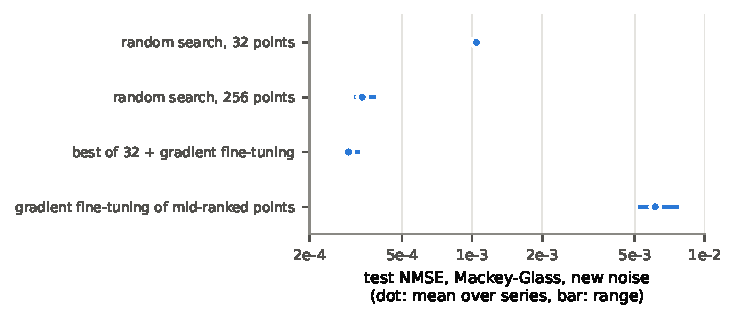
\includegraphics[width=0.75\linewidth]{fig7_gradient}
\caption{梯度微调与随机搜索的比较（现实噪声下的 Mackey--Glass，512 个模式、新噪声复测；点为 3 条序列的平均，横线为范围）。
从 32 个随机点中最好的点出发微调，与把随机搜索扩到 256 个点的结果相当；从排序中间的点出发，微调后仍远差于搜索。}
\label{fig:gradient}
\end{figure}

12 次微调全部好于各自的起点，误差降到起点的 0.24 到 0.93 倍，几何平均约 0.46 倍。
32 个随机点中最好的点为 $1.04\times10^{-3}$，从它出发微调后最好为 $2.9\times10^{-4}$；
而把随机搜索扩到 256 个点，直接得到 $3.4\times10^{-4}$，两者相当，差别在噪声实现之间的波动范围内。
另外三点限制了梯度微调的作用：
同一个起点换一个训练种子，结果相差近 2 倍（$2.9\times10^{-4}$ 对 $5.4\times10^{-4}$）；
从排序中间的点出发，微调后仍在 $6\times10^{-3}$ 以上，远差于搜索得到的点，也就是说微调救不了中等的起点；
12 次中有 3 次在最后一次验证（第 60 步）时仍是最好的，说明这几次还没有收敛，更长的训练可能还有收益。
计算量上随机搜索占明显优势：在同一块显卡上，每次微调（256 个模式、60 步）每步约 18 秒，一次约 18 分钟，从最好的 4 个起点出发的 8 次微调合计约 2.4 小时；
而把随机搜索从 32 个点扩到 256 个点，每条序列只多出一批批量仿真（一批最多 512 个工作点，约一到两分钟）。

所以在本文的参数规模下（约 70 个实数参数），单用随机搜索更划算；梯度微调最多适合作为搜索之后的精修，而且要换几个训练种子。
可微分仿真可能在两种情况下更有价值：一是可调的量很多（例如 64 根梳齿的掩模，或者多个环一起设计），随机搜索的效率会迅速下降，而梯度的代价几乎不变；
二是目标函数中有随机搜索难以覆盖的连续结构。这两点本文都没有检验。

\section{上限在软件坐标里的位置}\label{sec:software}

前几节一直以“现实噪声下、输入噪声 $3\times10^{-3}$ 的 31 节点 ESN”为软件对照。这个约定来自把激光强度噪声按调制深度折算到输入（第~\ref{sec:tasks}~节），
但它对结论的影响很大：表~\ref{tab:encodings} 中掩模与 ESN 在 Mackey--Glass 上持平（$3.3\times10^{-4}$ 对 $3.2\times10^{-4}$），
而 ESN 的输入噪声降到 $10^{-3}$ 时为 $5.3\times10^{-5}$，比掩模好约 6 倍，比加了读出侧改进的最好单环也好约 3 倍。
所以本节不取一个点，而是把软件的输入噪声从 0 扫到 $3\times10^{-3}$，把微环放到这条曲线上，回答“一个微环相当于多大、多吵的软件储备池”。

\subsection{软件输入噪声扫描}

图~\ref{fig:software} 给出 31、100、300 节点的 ESN（以及闭环任务中的 NG-RC~\cite{gauthier2021}）的测试误差随输入噪声的变化，协议与微环相同（第~\ref{sec:protocol}~节）；
微环取前几节中最好的结果，画成水平参考线。上方的横轴把输入噪声换算成模数转换器的有效位数：
若满量程对应输入信号的取值范围，$N$ 位量化的噪声均方根为 $2^{-N}/\sqrt{12}$，于是 $10^{-4}$、$3\times10^{-4}$、$10^{-3}$、$3\times10^{-3}$ 分别对应约 11.5、9.9、8.2、6.6 位。

\begin{figure}[htbp]
\centering
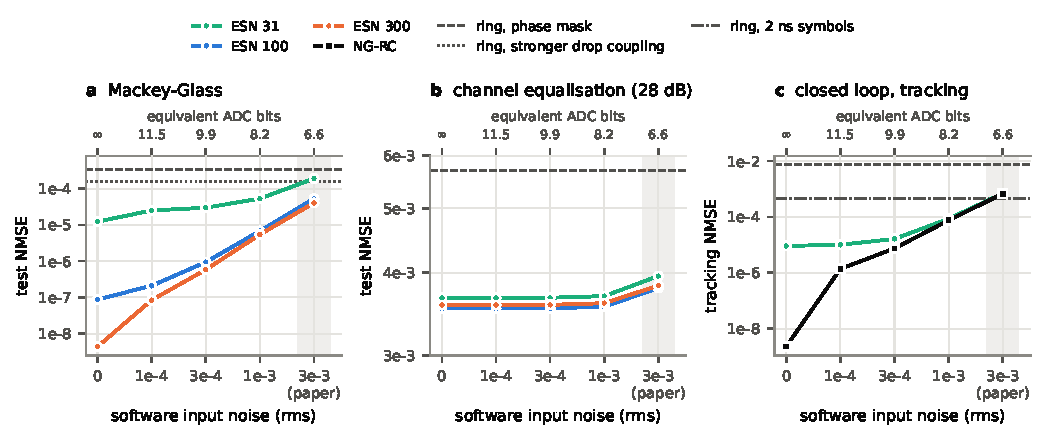
\includegraphics[width=\linewidth]{figS3_esn_input_noise}
\caption{软件储备池的测试误差随其输入噪声（均方根）的变化，上方横轴为等效的模数转换器有效位数 $N$（噪声 $2^{-N}/\sqrt{12}$）。
曲线：31、100、300 节点的 ESN 和 NG-RC（只在闭环任务中）；水平线：现实噪声下的微环（普通谱相位掩模、加大下载端口耦合、$2~\mathrm{ns}$ 符号）。
灰色带为前几节使用的约定值 $3\times10^{-3}$。（a）Mackey--Glass；（b）信道均衡（信噪比 $28~\mathrm{dB}$）；（c）闭环跟踪 Hénon 映射的指令轨迹（补充材料）。
与微环相同的选点和复测流程；Mackey--Glass 为 3 条序列的几何平均，信道均衡除 $3\times10^{-3}$ 外为单条序列，闭环为 4 组训练记录的平均。}
\label{fig:software}
\end{figure}

\emph{Mackey--Glass。} ESN 31 的误差在输入噪声为 0、$10^{-4}$、$3\times10^{-4}$、$10^{-3}$、$3\times10^{-3}$ 时为
$1.2\times10^{-5}$、$2.5\times10^{-5}$、$3.0\times10^{-5}$、$5.3\times10^{-5}$、$1.9\times10^{-4}$；
ESN 100 和 300 在 $3\times10^{-3}$ 时为 $5.3\times10^{-5}$ 和 $4.0\times10^{-5}$，无噪声时为 $8.8\times10^{-8}$ 和 $4.4\times10^{-9}$。
最好的单环（$1.55\times10^{-4}$）与 ESN 31 的交点在输入噪声约 $2.5\times10^{-3}$；100 和 300 节点的 ESN 在整个扫描范围内都更好，在 $3\times10^{-3}$ 时好 3 到 4 倍。

\emph{信道均衡、光纤链路和 NARMA-10。} 前两个任务的误差主要来自信道本身的噪声：ESN 31 的输入噪声从 $3\times10^{-3}$ 降到 0，误差只从 $3.95\times10^{-3}$ 降到 $3.66\times10^{-3}$，
ESN 增大到 300 个节点也几乎不变，但它们在整个扫描范围内都好于最好的微环（$5.7\times10^{-3}$）；
光纤链路上 ESN 为 $1.8\times10^{-2}$，微环最好为 $2.0\times10^{-2}$（补充材料）。
NARMA-10 上，即使在 $3\times10^{-3}$ 时 ESN 31、100、300 也为 $0.11$、$0.041$、$0.032$，好于单环的 $0.19$。

\emph{闭环决策。} 补充材料用微环预测 Hénon 映射的下一步，再按预测值施加有上限的控制。
跟踪一条指令轨迹时，$2~\mathrm{ns}$ 符号的微环跟踪误差为 $4.5\times10^{-4}$；
软件预测器的误差完全由它的输入噪声决定，与微环的交点约在 $2.4\times10^{-3}$，在 $10^{-3}$ 时 ESN 31 和 NG-RC 为 $8.6\times10^{-5}$ 和 $7.5\times10^{-5}$，好约 5 倍。
稳住不稳定平衡点只需要线性反馈，软件的模型能力不是限制，是最干净的标定：交点约在 $1.7\times10^{-3}$。

三个能直接比的任务给出一致的结论：最好的单环相当于输入噪声约 $1.7\times10^{-3}$ 到 $2.5\times10^{-3}$ 的 31 节点 ESN，
按上面的换算约合 \emph{7 位}（6.9 到 7.4 位）有效位数的模数转换器。

\subsection{7 位意味着什么}

这个数字要放在微环能工作的速率下看。本文的微环需要 $Q\sim10^{6}$ 才有足够的 Kerr 非线性，对应约 $0.5$ 到 $1~\mathrm{GBd}$ 的符号率。
这个速率下现成的模数转换器有约 9 位有效位数（例如采样率 $3.2~\mathrm{GSa/s}$ 的 12 位转换器，标称有效位数约 9 位~\cite{ti_adc12dj3200}）；
有效位数降到 5 到 6 位的是 $100~\mathrm{GSa/s}$ 以上、带宽几十吉赫兹的采集系统（例如带宽 $33~\mathrm{GHz}$ 时约 5.9 位、$110~\mathrm{GHz}$ 时约 5.0 位~\cite{keysight_uxr}），而那个速率下微环的 $Q$ 只能取 $2\times10^{4}$ 到 $4\times10^{4}$，Kerr 效应几乎用不上
（补充材料的光纤链路任务中，按 $28~\mathrm{GBd}$ 工作的微环只比线性均衡器好约 15\%）。也就是说，在微环能工作的速率下，把信号数字化后交给 31 节点的软件储备池，精度不会比微环差；
需要微环的场景只能是信号本来就在光域、数字化本身就是要省掉的那一步。

\subsection{读出端也要量化}\label{sec:quant}

上面把软件的输入噪声解读为模数转换器的量化噪声，但微环的 31 路读数同样要数字化，前面的结果都没有计入这一步。
为了让两边对称，我们在最好的单环上给每路读数各接一个 $N$ 位转换器（表~\ref{tab:quant}）。
满量程在拟合用的那次运行上按每路读数的范围标定一次，测试运行沿用这个标定，相当于先校准增益、再固定使用。
考虑两种接法：直接量化光电流的线性转换器，以及在转换器前加对数放大器（等比例的量化台阶，与读出层取对数一致）。
对照是 31 节点的 ESN，它的输入经 $N$ 位量化，不加其他噪声，也就是把软件那一侧的转换器换成真正的量化而不是等效的高斯噪声。

% generated by experiments/make_table3.py; do not edit by hand
\begin{table}[htbp]
\centering
\caption{读出端量化。最好的单环（加大下载端口耦合组，现实噪声，Mackey--Glass）的 31 路读数各接一个 $N$ 位模数转换器，满量程在拟合用的那次运行上按每路读数的范围标定一次，测试运行沿用；“线性”直接量化光电流，“对数”在转换器前加对数放大器。对照是输入经 $N$ 位量化、不加其他噪声的 31 节点 ESN（一个随机储备池）。3 条序列 $\times$ 6 对新运行的几何平均。不量化时微环为 $1.5\times10^{-4}$，无噪声的 ESN 为 $2.4\times10^{-5}$。}
\label{tab:quant}
\small
\begin{tabular}{cccc}
\toprule
位数 $N$ & 微环，线性转换器 & 微环，对数放大器 & ESN 31，输入量化 \\
\midrule
4 & $4.2\times10^{-3}$ & $1.9\times10^{-3}$ & $3.5\times10^{-3}$ \\
5 & $2.2\times10^{-3}$ & $1.1\times10^{-3}$ & $1.3\times10^{-3}$ \\
6 & $1.2\times10^{-3}$ & $5.6\times10^{-4}$ & $4.5\times10^{-4}$ \\
7 & $6.0\times10^{-4}$ & $3.5\times10^{-4}$ & $2.3\times10^{-4}$ \\
8 & $3.6\times10^{-4}$ & $2.7\times10^{-4}$ & $1.3\times10^{-4}$ \\
9 & $2.7\times10^{-4}$ & $2.1\times10^{-4}$ & $9.3\times10^{-5}$ \\
10 & $2.0\times10^{-4}$ & $1.8\times10^{-4}$ & $6.8\times10^{-5}$ \\
12 & $1.6\times10^{-4}$ & $1.6\times10^{-4}$ & $4.6\times10^{-5}$ \\
\bottomrule
\end{tabular}
\end{table}


微环需要较多的位数才不被量化拖累：两种接法都要 10 位，误差才回到不量化时（$1.54\times10^{-4}$）的 1.3 倍以内；
到 7 位时分别为 $6.0\times10^{-4}$ 和 $3.5\times10^{-4}$，差 2 到 4 倍。
原因在于梳齿功率跨越几个数量级，线性转换器分给弱梳齿的台阶很少；对数放大器缓解了这一点，但没有消除。
在 6 到 12 位的每一档，输入经同样位数量化的 ESN 都比 31 路都量化的微环好 1.2 到 3.4 倍（与带对数放大器的微环比；与线性转换器比差得更多）；
只有在 4 和 5 位这样很粗的量化下，带对数放大器的微环才好于 ESN，而那里两者的误差都在 $10^{-3}$ 以上。
另一个读法是：不量化的微环（$1.54\times10^{-4}$）落在输入量化 7 到 8 位的 ESN 之间（$2.3\times10^{-4}$ 和 $1.3\times10^{-4}$），与上一小节按等效噪声换算的约 7 位一致。

所以补上读出端的量化以后，比较只对微环更不利：软件只需要在输入端放一个转换器，而微环要 31 个，每个还要有约 10 位的有效位数。
在 $1~\mathrm{GBd}$ 下这样的转换器可以做到，但 31 路的功耗和成本是实际的代价。
如果在光域完成加权（用谱整形器加平衡探测直接算出读出层的线性组合），就只需要一个转换器；但延迟抽头这时要用光延迟线实现，本文没有模拟这种读出。

\subsection{多环阵列的上限}

单环的误差约一半来自它自己的失谐抖动和散粒噪声（第~\ref{sec:noise}~节），这两项在不同的环之间是独立的。
几个掩模不同的环共用一个输入光梳、读出拼接（每环 31 根梳齿 $\times$ 8 个抽头）时，这部分噪声会被平均掉。
训练长度加到 16 倍（16320 个符号）后，加大下载端口耦合的 1、2、4、8、16、32 个环为
$1.27\times10^{-4}$、$3.4\times10^{-5}$、$1.36\times10^{-5}$、$8.4\times10^{-6}$、$6.7\times10^{-6}$、$6.9\times10^{-6}$，
16 个环后不再下降，即误差降到单环的约 1/19 后饱和。
让所有环共用同一份激光强度噪声（同一个输入光梳分给所有环），结果几乎不变（16 个环为 $6.8\times10^{-6}$），说明饱和不是来自共模的光源噪声。
同样训练长度下，输入噪声 $3\times10^{-3}$ 的 ESN 100、300、1000 为 $3.9\times10^{-5}$、$2.1\times10^{-5}$、$1.4\times10^{-5}$，阵列好 2 到 3 倍；
但输入噪声降到 $10^{-3}$ 时（一条序列）为 $6.8\times10^{-6}$、$3.2\times10^{-6}$、$1.65\times10^{-6}$，100 节点的 ESN 已与 16 个环持平，1000 节点好约 4 倍。
所以阵列也只是把上限在软件坐标里往右移了一些，没有改变结论。
多环只在任务受各环自身噪声限制时有用：信道均衡在 $28~\mathrm{dB}$ 的信道噪声下加环和加大 ESN 都没有改善。

\subsection{为什么 $3\times10^{-3}$ 的约定偏严}

$3\times10^{-3}$ 是把激光强度噪声（$10^{-3}$）除以调制深度（$0.33$）得到的，相当于假设软件的输入和微环的输入一样吵。
但这一项在微环里的影响很小：第~\ref{sec:breakdown}~节中只打开激光强度噪声时，微环的误差只升高 1.5 到 1.9 倍；
而 ESN 31 在输入噪声 $10^{-4}$ 时就已经升高 2 倍。同一份强度噪声，对微环的伤害远小于把它折算成输入噪声后对 ESN 的伤害
（原因可能是强度噪声在微环里同时作用于泵浦和所有输入梳齿，部分表现为共模的变化，我们没有单独验证）。
所以 $3\times10^{-3}$ 对软件偏严，前几节中“与 ESN 31 持平”的说法都应理解为在这个偏严的约定下成立；
更公平的比较点在 $10^{-3}$ 附近，那里软件在本文的每个任务上都更好。

这一节的结论是：\emph{在本文考察的任务上，Kerr 微梳储备池的精度上限低于同规模的软件储备池；单个微环相当于输入接约 7 位模数转换器的 31 节点 ESN}。
评估协议是这个结论的一部分：只看一次噪声实现会乐观 10\% 到 30\%，混沌区的结果不可重复，给软件设的输入噪声能让比较翻转，所以我们给出整条曲线而不是一个点。

\section{讨论}\label{sec:discussion}

\subsection{实验实现}

消融结果（第~\ref{sec:ablation}~节）让实现大为简化：不需要逐梳齿的调制器。
一个与微环自由光谱范围锁定的 $200~\mathrm{GHz}$ 输入光梳分成两路，一路保持静态，另一路经过一个承载信号的强度或相位调制器；
两路各过一个只设相位（或幅度和相位）的谱整形器，分别写入式~\eqref{eq:mask} 中的偏置 $b_\mu$ 和权重 $w_\mu$，合束后与泵浦一起送入微环。
商用的硅基液晶谱整形器能独立设定各通道的幅度和相位，最窄通带约 $10~\mathrm{GHz}$、设定步长 $1~\mathrm{GHz}$，远小于梳齿间隔~\cite{coherent_waveshaper}；
C 波段的型号覆盖约 $5~\mathrm{THz}$（1527 到 $1568~\mathrm{nm}$），够 16 根输入梳齿（$3.2~\mathrm{THz}$），32 根以上要更宽的型号；
它的插入损耗（典型约 $5~\mathrm{dB}$，最大 6.5 到 $7~\mathrm{dB}$）要计入输入功率预算。
读出端是下载端口后的解复用器加 31 个光电探测器，结构与频率复用的光学储备池~\cite{butschek2020,lupo2023} 相同。
最难的部分是输入光梳本身：它要与微环的自由光谱范围对齐，并且相位稳定；本文没有模拟它的噪声。

光源的要求来自第~\ref{sec:laser}~节：泵浦激光相对于谐振的本征线宽要在几千赫兹以下。
这排除了普通的 DFB 激光（$100~\mathrm{kHz}$ 到 $1~\mathrm{MHz}$），需要窄线宽激光或自注入锁定~\cite{shen2020}。
慢的频率漂移（远长于一个符号）则要靠锁定环路压到半线宽的约 0.3\% 以内，否则训练好的读出层会随漂移失效（补充材料的闭环实验中，1\% 的慢漂移已让跟踪误差变差 2.4 倍）。

\subsection{功耗与速率}

最好的单环需要约 $180~\mathrm{mW}$ 的总输入光功率（加大下载端口耦合组），其余掩模的最优点在约 20 到 $200~\mathrm{mW}$ 之间；
换成 Si$_3$N$_4$ 微环可以降到约 1/4，但到达探测器的光同样变少，要配更好的探测器或光放大器（第~\ref{sec:platform}~节）。
速率被 Kerr 非线性所需的 $Q$ 限制在约 $1~\mathrm{GBd}$。
以 $1~\mathrm{GBd}$、$180~\mathrm{mW}$ 计，每个符号的光能约 $180~\mathrm{pJ}$，还没有计入激光器的电光转换效率、31 路探测和读出层的计算。
我们没有把它和数字电路做能耗比较，因为那需要一个具体的系统场景，而本文的结论（第~\ref{sec:software}~节）是在精度上微环不占优，能耗上的好处也就只能在信号本来在光域、数字化可以省掉的场景里讨论。

\subsection{局限}

\emph{全部是仿真。} 本文的结论依赖 LLE 模型和噪声模型。我们按规格书和文献选了探测器噪声（每根梳齿 $0.3~\mu\mathrm{W}$，位于 1~GHz 级 InGaAs PIN 接收机 0.13 到 $0.63~\mu\mathrm{W}$ 的中间）、
激光强度噪声和频率噪声，并对后者按真实频谱复核；但微环的热折射噪声、光放大器的自发辐射自拍频、探测器量子效率和输入光梳的噪声都没有建模。
对文献方案的复现也有不确定性：原文没有给出腔长、$Q$ 的分配和采样间隔，我们的对比应理解为“在本文的实现中”。

\emph{读出端。} 读出端的量化只在最好的单环上、用一种标定方式算过（第~\ref{sec:quant}~节）；在光域完成加权的读出没有模拟。

\emph{任务。} 三个基准任务和一个光纤链路任务都是标准任务，掩模的优势集中在需要强非线性、短记忆的预测上；需要长记忆的任务要靠外加延迟线（第~\ref{sec:memory}~节）。

\subsection{试过但不成立的方向}

为了寻找微环相对软件的优势，我们还试了几个方向，结果都是否定或有限的，这里简述，以免后来者重复：
\begin{itemize}
\item \emph{闭环决策}（补充材料）：微环预测 Hénon 映射、再据此控制。微环能在闭环里工作，决策质量由预测噪声决定；
      它只在软件输入噪声取 $3\times10^{-3}$ 时略好于 ESN 和 NG-RC，低于约 $2.4\times10^{-3}$ 时不再领先。
\item \emph{用微环控制另一个 Kerr 微环}：被控对象换成单模 Kerr 腔后，微环控制器的跟踪误差（$0.023$）与 ESN 31（$0.023$）和带前馈的比例微分控制器（$0.022$）相同，
      只比单纯的比例微分控制器（$0.068$）好约 3 倍；稳住不稳定态时，比例微分控制器和 ESN 的成功率（94\% 和 91\%）都高于微环（68\%）。
\item \emph{共参考环}：用一个不加信号的环测出共模的失谐抖动并在读出端减掉。理想参考下也只降 2\%，见第~\ref{sec:reference}~节。
\item \emph{传感}：用同一个光梳估计外加的失谐偏移（以半线宽为单位的均方根误差）。
      窄量程（$\pm0.3$ 个半线宽）内，31 根梳齿的光梳读出只比低功率泵浦加参考的经典读法好约 1.5 倍（$1.0\times10^{-3}$ 对 $1.5\times10^{-3}$）；
      宽量程（$\pm2$ 个半线宽）内光梳远好于只读泵浦（$0.07$ 到 $0.09$ 对 $0.5$ 以上），但几乎没有 Kerr 效应的低功率光梳更好（$0.042$），
      说明好处来自多根梳齿同时探测，而不是 Kerr 非线性。
\end{itemize}
这些结果和第~\ref{sec:software}~节一致：在精度上，Kerr 微梳储备池能做到的是接近一个小型、带量化噪声的软件储备池；
它的价值只能来自物理层（信号本来在光域、延迟、能耗），本文没有证明这一点，我们把它作为后续工作的问题提出。

\section{结论}\label{sec:conclusion}

我们在统一的评估协议下用仿真研究了一个问题：在现实噪声下 Kerr 微梳储备池表现如何、受什么限制、和软件相比处在什么位置。

第一，编码很重要。给输入光梳的每根梳齿加上随机复权重再送入微环，得到输出由输入决定、而不是由起振噪声决定的相干种子区。
在相同的物理条件和选点预算下，这种谱相位掩模在 Mackey--Glass 预测上比整体调制的光梳好一到两个数量级、比我们实现的单泵浦编码好两到三个数量级，
在信道均衡上与整体调制的光梳相当，单环在 NARMA-10 上没有帮助。梳齿相位的随机性比逐梳齿的幅度更重要，所以一个调制器加两个谱整形器就够了。
线性腔对照表明，Mackey--Glass 上的好处主要来自 Kerr 动力学；信道均衡上所需的非线性由相互干涉的输入梳齿经探测提供，Kerr 项没有贡献。

第二，下限由噪声决定，其中约一半在光源。理想探测器下误差下限约一半来自失谐抖动、一半来自散粒噪声；换 Si$_3$N$_4$ 或加功率都降不了它，
读出侧的改法（加大下载端口耦合、放慢符号）能降一部分。把真实抖动序列交给线性读出层没有去掉抖动，重新选工作点也没有绕开它，
所以本文器件的激光本征线宽要在几千赫兹以下；$100~\mathrm{kHz}$ 的普通激光让最好的单环比用 $1.6~\mathrm{kHz}$ 激光时差 5 到 6 倍。记忆要靠外加的延迟线和读出抽头。

第三，在软件坐标里，找到的最好微环低于同规模软件。它相当于输入接约 7 位转换器的 31 节点 ESN，而在微环能工作的约 $1~\mathrm{GBd}$ 下，现成的转换器有约 9 位；
把微环 31 路读数的量化也算进去后，在 6 到 12 位的每一档，只在输入端量化的 ESN 都更好。
16 个环拼接读出能把误差再降约 19 倍，但输入噪声更低的大型软件储备池同样能追平。
这个比较对给软件设定的输入噪声很敏感，所以我们给出整条曲线，并建议后续工作都这样报告。

第四，信号和抖动看来作用在同一个量（有效失谐）上，我们考察的工作点都避不开抖动。用反相信号同时驱动同一微环的两个方向（我们初步把好处归于交叉相位耦合），
读出两个方向并优化掩模，误差达到 $7.3\times10^{-6}$，比最好的单向微环低 21 倍，比同样读出、同样优化的单向微环低 4.5 倍；与输入权重得到同样优化的 62 节点 ESN 相比约为 8 位，比之前多 1 位，但仍低于这一速率下现成转换器的精度。

因此在本文探索的设计空间内，Kerr 微梳储备池的理由不在计算精度上。它能否落在物理层（信号本来在光域、省掉数字化、配合光域加权的延迟和能耗）上，本文没有检验；
这需要一个具体的光域应用、一次实验，以及在光域完成加权、只用一个转换器的读出方案。


\section*{代码与数据}
仿真器（\texttt{combrc}）、全部实验脚本、每张表和图所依据的结果汇总以及生成它们的脚本，按 MIT 许可公开在
\url{https://github.com/changxvdu-source/kerr-comb-reservoir}。

\bibliographystyle{unsrtnat}
\bibliography{refs}

\end{document}
